% !TEX program = xelatex
\documentclass[usenames,dvipsnames,aspectratio=169]{beamer}

\usefonttheme{professionalfonts}
\usepackage[no-math]{fontspec}
\usepackage{multicol}

\usepackage[none]{hyphenat}
\usepackage{hyperref}

\fontspec [Path = ./fonts/, 
    UprightFont = TextbookNew-Light,
    BoldFont = TextbookNew-Regular]
{Textbook New}

\defaultfontfeatures{Scale=MatchLowercase}
\setmainfont[Path=fonts/,
    UprightFont = TextbookNew-Light,
    BoldFont = TextbookNew-Regular,
%   ItalicFont = TextbookNew-LightItalic,
%   BoldItalicFont = TextbookNew-Italic
]{Textbook New}
\setromanfont[Path=fonts/,
    UprightFont = TextbookNew-Light,
    BoldFont = TextbookNew-Regular
%   ItalicFont = TextbookNew-LightItalic,
%   BoldItalicFont = TextbookNew-Italic
]{Textbook New}
\setsansfont[Path=fonts/,
    UprightFont = TextbookNew-Light,
    BoldFont = TextbookNew-Regular
%   ItalicFont = TextbookNew-LightItalic,
%   BoldItalicFont = TextbookNew-Italic
]{Textbook New}
\setmonofont[Path=fonts/, UprightFont = InputMono-Regular]{Input Mono}
\newfontfamily{\cyrillicfont}[ Path=fonts/ ]{TextbookNew-Light}
\newfontfamily{\cyrillicfontbf}[ Path=fonts/ ]{TextbookNew-Regular}
\newfontfamily{\cyrillicfonttt}[Path=fonts/, UprightFont = InputMono-Regular]{Input Mono}

\usepackage{yandex}
\usepackage{amsmath,amssymb,amsfonts,amsthm}
\usepackage{mathtools}

\setdefaultlanguage{english} % язык определяет перевод названий, в том числе и логотипа

\title{Intro into Machine Learning}
\subtitle{Fifth Machine Learning in High Energy Physics Summer School,\\
MLHEP 2019, August 1--10}

\author[Alexey Artemov]{
  Alexey Artemov$^{1, 2}$
}
\institute{
    \begin{tabular}{c c}
        $^1$~Skoltech &
        $^2$~Higher~School~of~Economics
    \end{tabular}
}

\onbehalf{Linear Models. Numerical optimization. Logistic Regression. Figures of Merits. Overfitting. Model Selection. Regularization. }

\noyandexlogoframe


%%%%%%%%%%%%%%%%%%%%%%%%%%%%%
\usepackage{graphicx}
\DeclareGraphicsExtensions{.eps,.png}
\graphicspath{ {img/} }

% \usefonttheme[onlymath]{serif}

% added by Evgeny Sokolov
\def\XX{\mathbb{X}}
\def\PP{\mathbb{P}}
\def\FF{\mathcal{F}}
\def\EE{\mathbb{E}}
\def\NN{\mathcal{N}}
\def\LL{\mathcal{L}}
\def\YY{\mathbb{Y}}
\def\RR{\mathbb{R}}
\def\HH{\mathbb{H}}
\def\AA{\mathcal{A}}
\newcommand{\cond}{\mspace{3mu}{|}\mspace{3mu}}
\newcommand{\argmin}{\mathop{\rm arg\,min}\limits}

\usepackage{tikz}
\usetikzlibrary{positioning,arrows,shapes.geometric,shadows,trees}
\usetikzlibrary{calc}

\tikzstyle{format} = [thick, draw=red!50!black!50]
\usepackage{tkz-graph}

\usepackage{color}
\usepackage{bm}
\usepackage{animate}

\setlength{\abovedisplayskip}{2mm}
\setlength{\belowdisplayskip}{2mm}
%%%%%%%%%%%%%%%%%%%%

\begin{document}

% Несколько альтернатив основного логотипа на титульную страницу:
%\yandexlogo                          % общий логотип Яндекса
%\yandexservicelogo{Название сервиса} % логотип конкретного сервиса

%\yandexschoollogo                    % логотип ШАД
% \crayfislogo
%\yandexdatafactorylogo               % логотип YDF

% Дополнительные логотипы. Здесь можно указывать произвольный код. \textheight обозначает допустимую высоту.
\addlogo{
\includegraphics[height=\textheight,keepaspectratio]{yandex/hse.eps}}
\addlogo{
\includegraphics[height=\textheight,keepaspectratio]{yandex/logo_shad.eps}}
\addlogo{
\includegraphics[height=\textheight,keepaspectratio]{yandex/logo_skoltech.png}}
% \addlogo{
\includegraphics[height=\textheight,keepaspectratio]{yandex/mipt.eps}}
% \addlogo{
\includegraphics[height=\textheight,keepaspectratio]{yandex/st.png}}
% \addlogo{
\includegraphics[height=\textheight,keepaspectratio]{yandex/ucd_seal.eps}}
% \addlogo{
\includegraphics[height=\textheight,keepaspectratio]{yandex/uci.eps}}
% %\addlogo{\insertyandexdataschoollogo[height=\textheight,keepaspectratio]}
% %\addlogo{\insertyandexdatafactorylogo[height=\textheight,keepaspectratio]}


\begin{frame}[plain]
\titlepage
\end{frame}


\begin{frame}
\frametitle{Lecture overview}

% \tableofcontents

% \huge \textcolor{red}{TODO: REPLACE BY CONTENTS}

% \normalsize
\begin{itemize}

\item Linear models for regression
\item Numerical and stochastic optimization at a glance 
\item Linear models for classification
\item Figures of merits
\item Overfitting: how to fool the linear regression
\item Regularization
\item A Bayesian perspective on regularization
\end{itemize}

\end{frame}



% \section{Machine learning in~high energy physics}



% \begin{frame}
% \frametitle{Search for the exotic particles in HEP}

% \begin{columns}
% \begin{column}{0.65\textwidth}
%     \begin{itemize}

%     \item Starred in the \textbf{HIGGS benchmark} 

%     \item \textbf{The goal:} classify \textcolor{Plum}{signal} vs. \textcolor{orange}{background} processes

%     \begin{center}
%      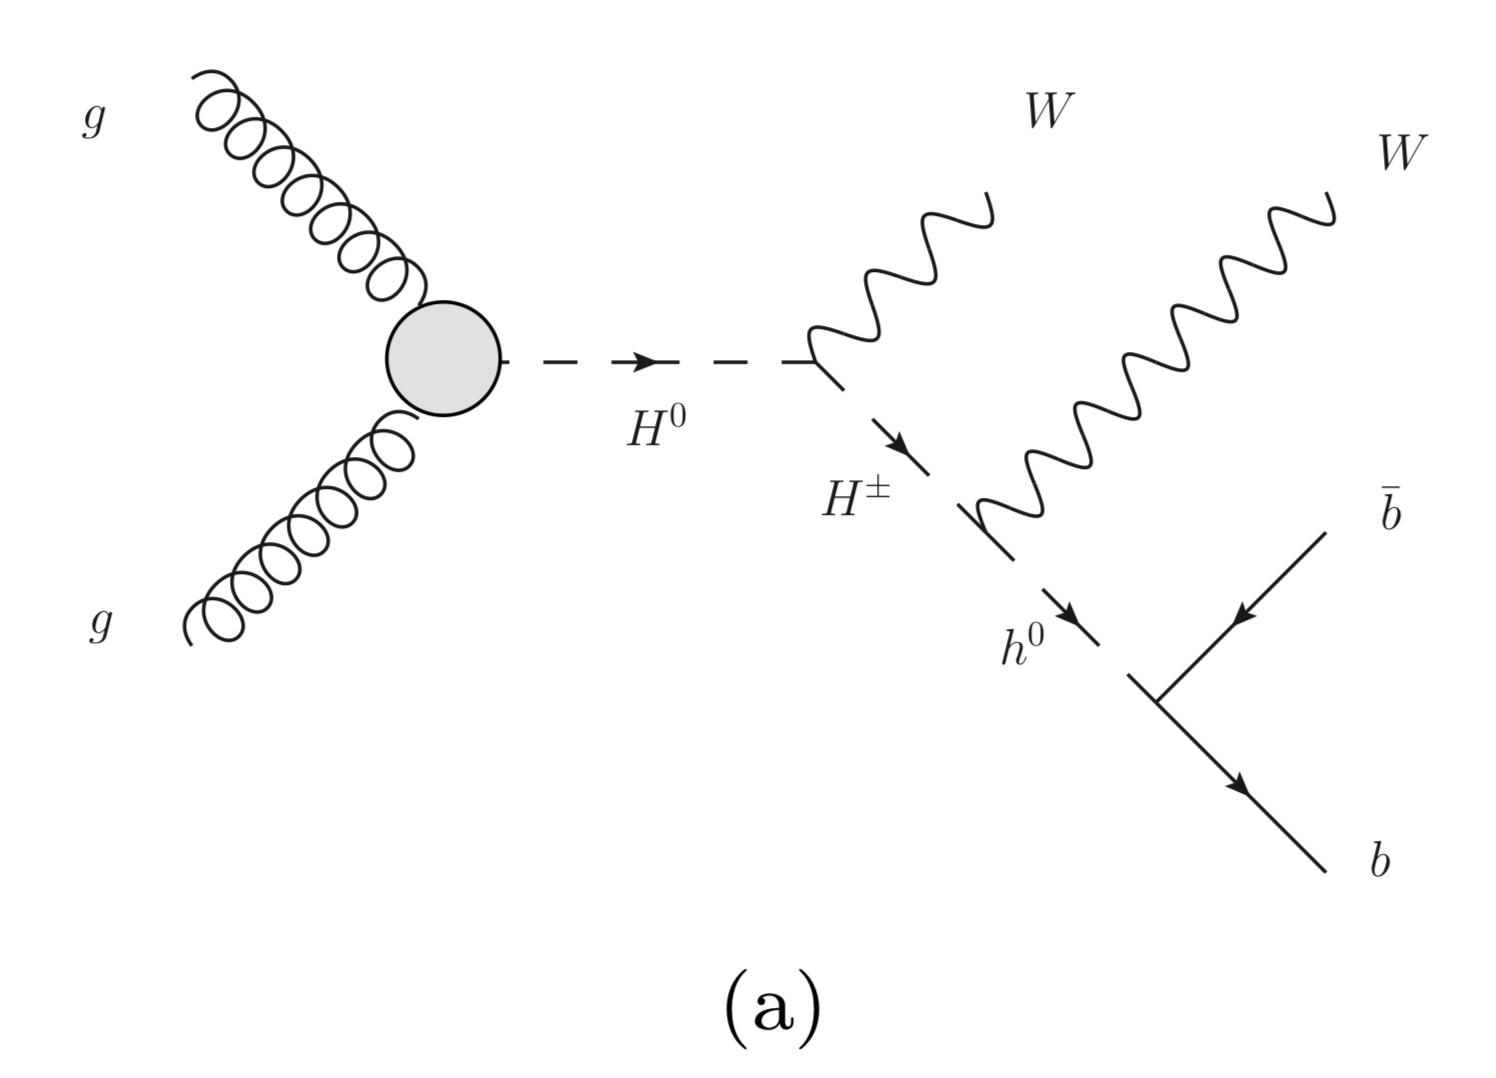
\includegraphics[width=0.4\columnwidth]{higgs_type1.png}
%      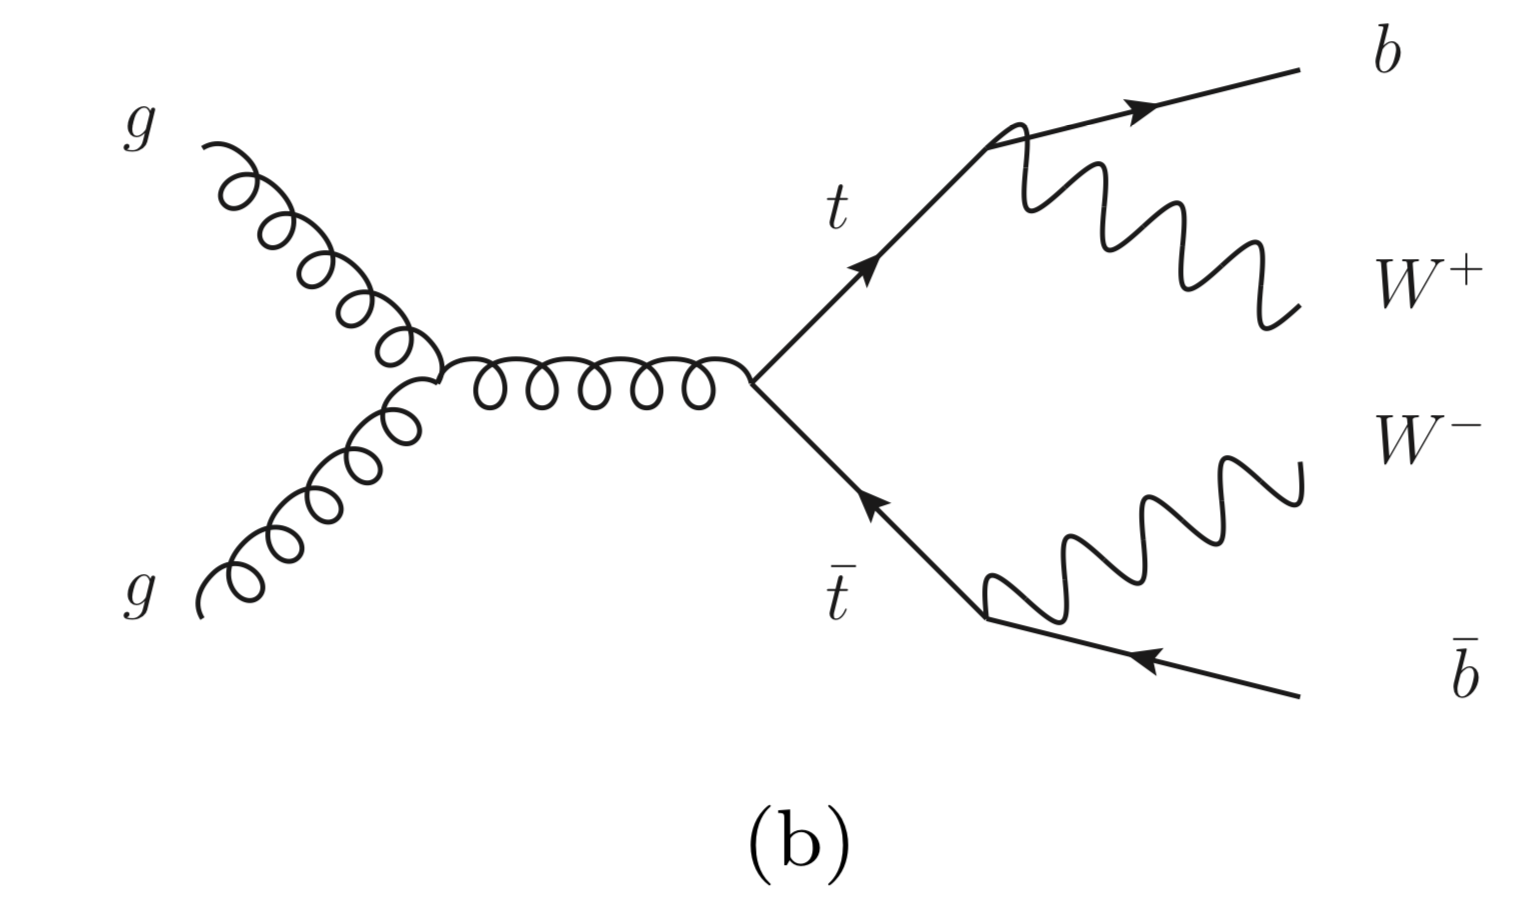
\includegraphics[width=0.4\columnwidth]{higgs_type2.png}
%      \end{center}

%   \item Features: jets 1 through 4 $p_T$s, 
%     lepton $p_T$, missing transverse momentum, etc.
%     (28 features in total)

%     \item Dataset size: 11 mln events
%     (\url{http://archive.ics.uci.edu/ml/datasets/HIGGS})

%     \end{itemize}


% \end{column}
% \begin{column}{0.35\textwidth}  %%<--- here

%      \begin{center}
%      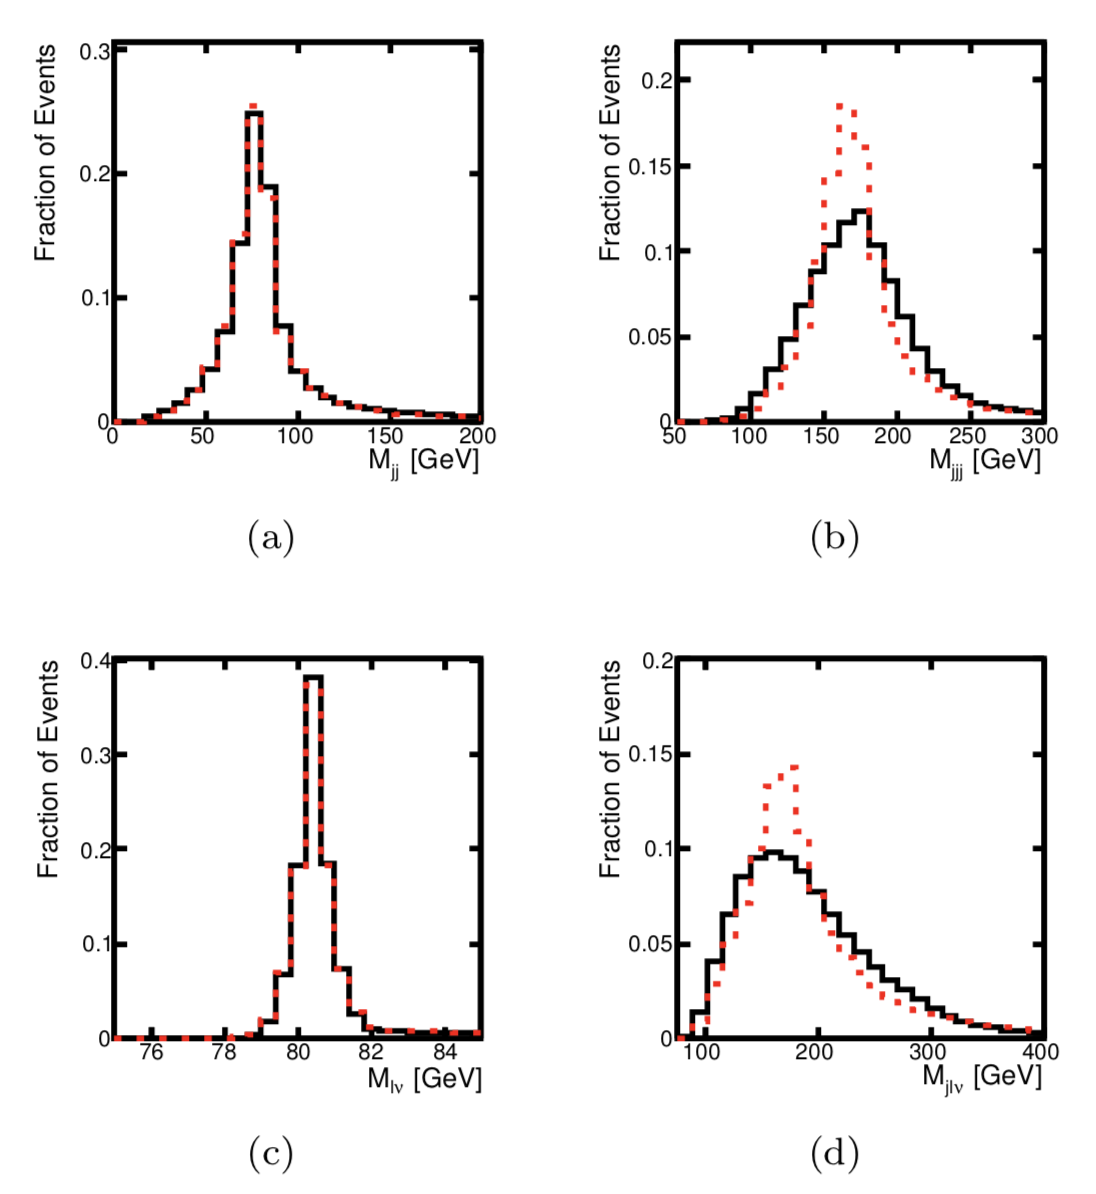
\includegraphics[width=1.1\columnwidth]{higgs_features.png}
%      \end{center}


% \end{column}
% \end{columns}

% \end{frame}



% \begin{frame}
% \frametitle{Machine learning for the real world}

% \huge \textcolor{red}{TODO: REPLACE BY HIGGS}

% % \begin{columns}
% % \begin{column}{0.5\textwidth}

% % \begin{itemize}
% %     \item Use stats!

% %     \item Properties and revenues
% %     of existing restaurants:
% % \end{itemize}

% % \begin{table}[h]
% %   \centering
% %   % \resizebox{\textwidth}{!}{%
% %   \begin{tabular}{@{} l l l @{}}
% %   \textbf{Id} & \textbf{Location}    & \textbf{Revenue} \\ 
% %   \hline
% %   1            & 51.472866,-0.2588277  & \$1.1M \\
% %   2            & 51.4865675,-0.2210999 & \$2.23M \\
% %   $\ldots$            & $\ldots$ & $\ldots$ \\
% %   20           & 51.4334641,-0.5146408 & \$0.59 \\
% %   \end{tabular}
% %   % }
% % \end{table}

% % \end{column}
% % \begin{column}{0.5\textwidth}  %%<--- here
% %     \begin{center}
% %      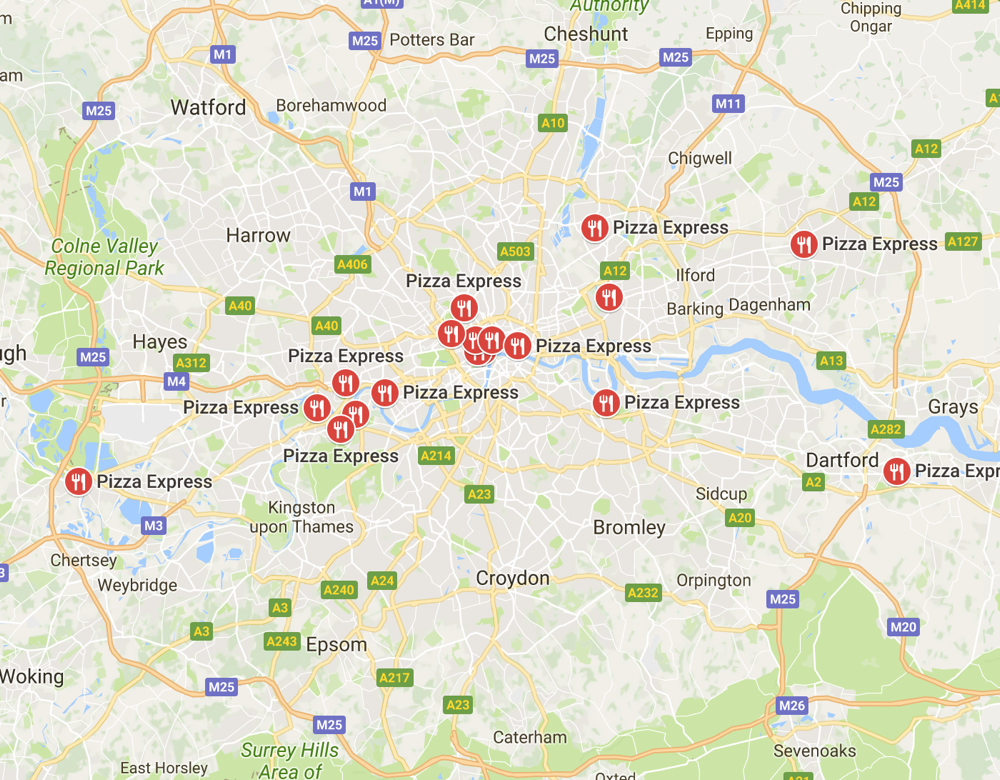
\includegraphics[width=0.9\columnwidth]{intro-pizza.png}
% %      \end{center}
% % \end{column}
% % \end{columns}

% \end{frame}



% \begin{frame}
% \frametitle{Some notation}

% \huge \textcolor{red}{TODO: REPLACE BY HIGGS FEATURES}

% \normalsize

% \begin{itemize}

%     \item Object space $\mathbb{X} = \mathbb{R}^2$:
%     restaurant location
% (also known as the feature space)

%     \item Target space $\mathbb{Y} = \mathbb{R}$:
%     restaurant revenue

%     \item Training set $X^{\ell} = 
%     \big\{(\mathbf{x}_i, y_i)\big\}_{i=1}^{\ell}$
%     (known locations and revenues for existing restaurants)

%     \item \textbf{The goal:} estimate $y \in \mathbb{Y}$ 
%     for a new $\mathbf{x} \in \mathbb{X}$
%     (estimate revenue for a proposed location)

% \end{itemize}

% \end{frame}



\begin{frame}
\frametitle{``Physics-based'' vs. machine-learned models}

\begin{itemize}

    \item Some criteria for machine learning to be applied in a dependency recovery setting:
    \begin{itemize}
        \pause
        \item Little prior knowledge of the dependency exists
        \pause
        \item The dependency has a complex form too hard for manual examination
        \pause
        \item A sample from the dependency of sufficiently large size is available
    \end{itemize}

\end{itemize}

\end{frame}



\begin{frame}
\frametitle{``Physics-based'' vs. machine-learned models}

\begin{itemize}

    \item Would one want to apply machine learning for $\ldots$
    \begin{itemize}
        \pause 
        \item $\ldots$ Newton’s mechanics?
        \pause
        \item $\ldots$ suggesting music to radio listeners?
        \pause
        \item $\ldots$ sorting integers?
        \pause
        \item $\ldots$ controlling steel production?
        \pause
        \item $\ldots$ sorting strawberries?
    \end{itemize}

\end{itemize}

\end{frame}



% \begin{frame}
% \frametitle{What is machine learning about?}

% \begin{itemize}

%     \item Inference of statistical dependencies which give us ability to predict

%     \item Data is cheap, knowledge is precious 

% \end{itemize}

% \huge \textcolor{red}{add physics-related diagram}

% \begin{center}
%   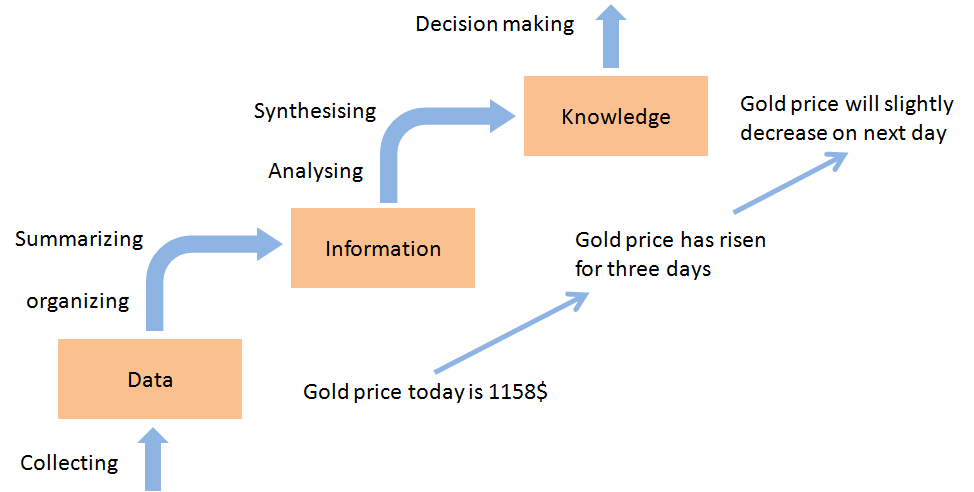
\includegraphics[width=0.7\columnwidth]{data-to-knowledge.png}
% \end{center}

% \vspace{-4mm}
% \begin{flushright}
% {\footnotesize \textcolor{gray}{Picture credit: 
% https://www.packtpub.com/books/content/introduction-data-analysis-and-libraries}}
% \end{flushright}


% \end{frame}



% \begin{frame}
% \frametitle{Feature vectors}

% \huge \textcolor{red}{replace by higgs features and other features from physics}
% \normalsize
% \begin{itemize}

%     \item Computers cannot operate objects of the real world directly

%     \item Need \textcolor{orange}{\textbf{features}} describing the objects
%     ($\mathbf{x} = (\mathrm{lat}, \mathrm{lon})$ for the restaurant)

% \end{itemize}

% \begin{columns}
% \begin{column}{0.35\textwidth}

% \pause
% \begin{itemize}
% \item In real applications such as fraud detection, 
% \textcolor{Fuchsia}{feature engineering} is the most
% complex task
% \item Many papers on the problem
% \end{itemize}

% \vspace{-5mm}
% \begin{center}
%   
\includegraphics[width=0.6\columnwidth]{credit_card_fraud.png}
% \end{center}

% \end{column}
% \begin{column}{0.65\textwidth}

% \pause
% \begin{itemize}
% \item Machine location (e.g. beside supermarket, latitude, longitude), brand, and age
% \item Customer demographic (e.g. postcode) and behavioral information
% \item Card type (e.g. Visa, supplementary, issued yesterday) and usage
% \item Session/transaction day-of-week, time-of-day, keystrokes (e.g. number of login attempts), transaction type, and amount
% \end{itemize}

% \end{column}
% \end{columns}

% \end{frame}



% \begin{frame}
% \frametitle{Possible kinds of features: some more notation}

% {\huge
% \textcolor{red}{
%   add higgs features and other features from physics}
% \par}

% \begin{itemize}

% \item Binary: $x\in\{0, 1\}$ \textit{(are you a member of a terrorist organization?)}
% \item Real-valued: $x \in \mathbb{R}$ (customer income)
% \item Categorical: $x \in S$ where $|S| = n$
% and order of elements in $S$ does not matter
% (customer postcodes)
% \item Ordinal: $x \in S$ where $|S| = n$
% and order of elements in $S$ does matter\\
% (old < renovated < new for house price prediction)
% % \item Set-valued 
% \item Structured: images (customer photo in the fraud detection task)

% \end{itemize}

% \end{frame}



% \begin{frame}
% \frametitle{Kinds of machine learning tasks}

% {\huge
% \textcolor{red}{replace stupid picture with something meaningful}
% \par}

% \begin{columns}
% \begin{column}{0.55\textwidth}

% \begin{itemize}
% \only<1->{
% \item Supervised learning 
% }
% \only<2->{
%     \begin{center}
%     \begin{tikzpicture}[>=latex,->,scale=0.7, every node/.style={scale=1.0}]
%       \tikzset{stat/.style={fill=blue!20,
%       draw=blue!75, minimum size=.75cm}}
%       \tikzset{stoptime/.style={fill=yellow!20,
%        draw=brown!75, minimum size=.75cm}}

%       \node[stat] (data) [align=center,text width=2cm] at (0,0)
%         {data};
%       \node[stat] (resp) [below=6mm of data,align=center,text width=2cm] at (0,0)
%         {responses};
%       \node[stoptime] (model) [below right=.0cm and 1cm of data,align=left]
%         {model};

%         \path[->] (data) edge (model);
%         \path[->] (resp) edge (model);
%     \end{tikzpicture}
%     \end{center}
% }
% \only<3->{
%     \vspace{-2.5mm}
%     \begin{itemize}
%         % \large
%     \item Regression, (multi-class/multi-label) classification, semi-supervised learning
%     \end{itemize}
% }

% \only<5->{
% \item Unsupervised learning
% }
% \only<6->{
%     \begin{center}
%     \begin{tikzpicture}[>=latex,->,scale=0.7, every node/.style={scale=1.0}]
%       \tikzset{stat/.style={fill=blue!20,
%       draw=blue!75, minimum size=.75cm}}
%       \tikzset{stoptime/.style={fill=yellow!20,
%        draw=brown!75, minimum size=.75cm}}

%       \node[stat] (data) [align=center,text width=2cm] at (0,0)
%         {data};
%       \node[stoptime] (structure) [right=1cm of data,align=left]
%         {data structure};

%         \path[->] (data) edge (structure);
%     \end{tikzpicture}
%     \end{center}
% }
% \only<7->{
%     \vspace{-2.5mm}
%     \begin{itemize}
%         % \large
%     \item Clustering, density estimation, dimensionality reduction, visualization

%     \end{itemize}
% }
% % \item Reinforcement learning

% \end{itemize}


% \end{column}
% \begin{column}{0.45\textwidth}

% \only<4->{
% \begin{center}
%     
\includegraphics[width=0.75\columnwidth]{intro-mltasks-supervised.png}
% \end{center}
% }

% \only<8->{
% \begin{center}
%     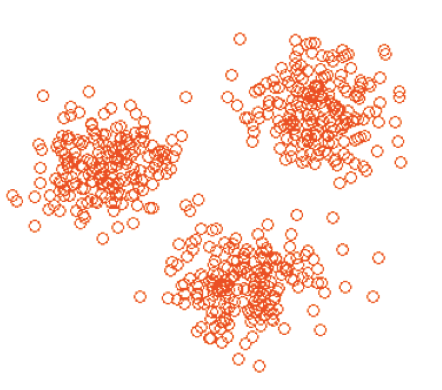
\includegraphics[width=0.55\columnwidth]{intro-mltasks-unsupervised.png}
% \end{center}
% }

% \end{column}
% \end{columns}


% \end{frame}



\begin{frame}
\frametitle{Machine learning as function approximation}

\begin{itemize}

\item An unknown distribution $D$
generates \textcolor{Plum}{instances} ($\mathbf{x}_1, \mathbf{x}_2, \ldots$)
independently

\pause
\item An unknown function 
$f: \mathbb{X} \to \mathbb{Y}$ generates \textcolor{Plum}{responses}
($y_1, y_2, \ldots$) for them
such that $y_i = f(\mathbf{x}_i), i=1, 2, \ldots$

\pause
\item The machine learning problem:
choose a plausible \textcolor{Plum}{hypothesis} 
$h: \mathbb{X} \to \mathbb{Y}$
from the \textcolor{Plum}{hypothesis space} $\mathbb{H}$

% \item $h \in \mathbb{H}$ is the learner's output

\pause
\item The error of a hypothesis $h$ is 
the deviation from the true $f$
measured by the \textcolor{Plum}{loss function} (an example for regression):
\[
    Q(h, X^{\ell}) = \frac {1} {\ell} 
    \sum\limits_{i=1} ^{\ell} 
        (f(\mathbf{x}_i) - h(\mathbf{x}_i))^2
\]

\pause 
\item \textcolor{orange}{\textbf{Learning:}} the search for the optimal 
hypothesis $h \in \mathbb{H}$ 
w.\,r.\,t. the fixed loss function

\end{itemize}

\end{frame}



\begin{frame}
\frametitle{Function approximation: energy usage}

\vspace{-10mm}
\begin{columns}[t]
\begin{column}{0.225\textwidth}

    \vspace{10mm}
    \only<2->{\large instances?}

    \vspace{10mm}
    \only<2->{\large responces?}

    \vspace{10mm}
    \only<3->{\large hypothesis?}
\end{column}


\begin{column}{0.5\textwidth}

    \begin{center}
    \begin{figure}[t!]
        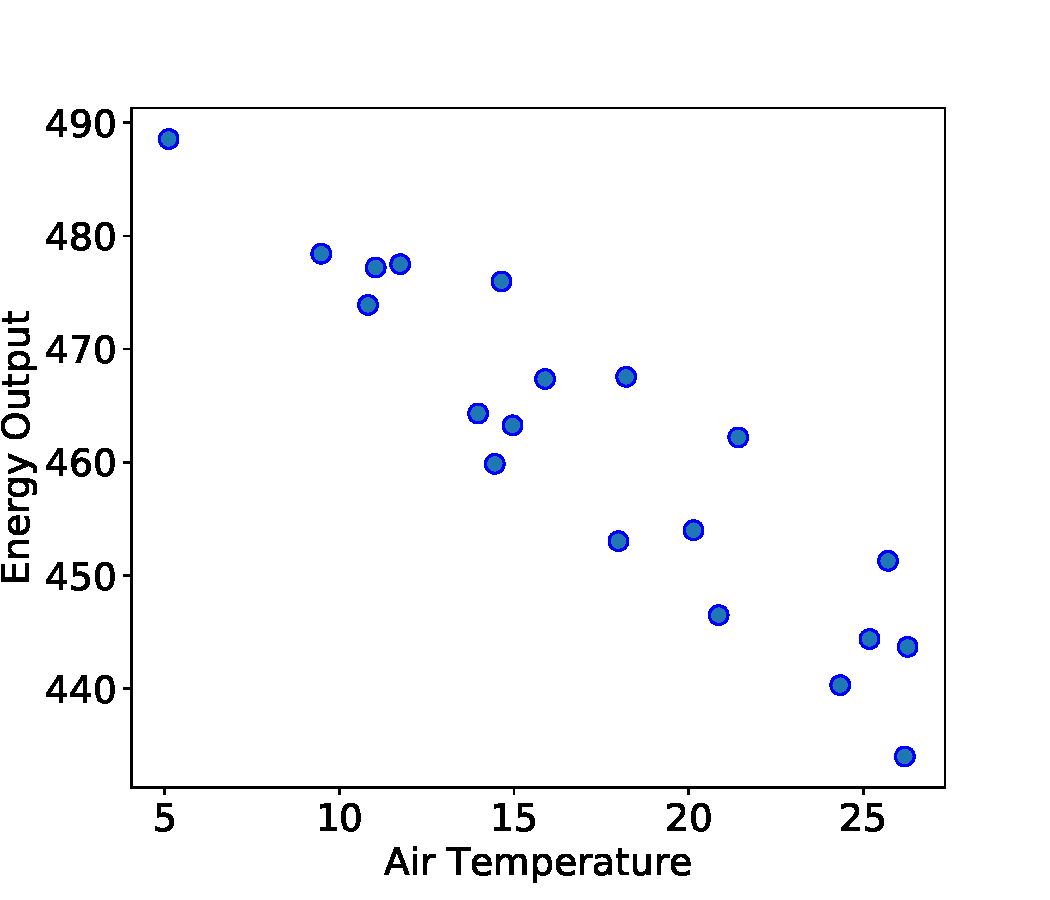
\includegraphics[
        width=\columnwidth,
        trim=0mm 0mm 10mm 10mm,
        clip=True]
        {univariate_scatter.pdf}
    \end{figure}
    \end{center}

\end{column}

\begin{column}{0.275\textwidth}

    \vspace{10mm}
    \only<4->{\large loss?}

    \vspace{10mm}
    \only<5->{\large learning?}

    \vspace{10mm}
    \only<6->{\large approximation?}
\end{column}


\end{columns}


\begin{itemize}
    \item {\bf The goal:} obtain some fit $f(x)$
    plausible for every $x_i$ and $y_i$

\end{itemize}

\end{frame}



% \begin{frame}
% \frametitle{The machine learning pipeline}

% {\huge
% \textcolor{red}{add description for all boxes, revise them}
% \par}

%     \begin{center}
%     \begin{tikzpicture}[>=latex,->,scale=0.7, every node/.style={scale=1.0}]
%       \tikzset{nodestyle/.style={fill=yellow!20,
%        draw=brown!75, minimum size=.75cm}}

%       \node[nodestyle] (setup) [align=left,text width=2.5cm] at (0,0)
%         {1. Setup\\the problem};
%       \node[nodestyle] (features) [right=1cm of data,align=left,text width=2.5cm]
%         {2. Engineer\\features};
%       \node[nodestyle] (sample) [right=1cm of features,align=left,text width=2.5cm]
%         {3. Form\\a sample};

%       \node[nodestyle] (quality) [below right=5mm and 0cm of sample,align=left,text width=3cm]
%         {4. Choose\\quality metrics};

%       \node[nodestyle] (preprocess) [below=25mm of sample,align=left,text width=3cm]
%         {5. Preprocess\\the sample};
%       \node[nodestyle] (learn) [left=1cm of preprocess,align=left,text width=2.5cm]
%         {6. Learn\\the model};
%       \node[nodestyle] (eval) [left=1cm of learn,align=left,text width=2.5cm]
%         {7. Evaluate\\quality};

%         \path[->] (setup) edge (features);
%         \path[->] (features) edge (sample);
%         \path[->] (sample) edge (quality);

%         \path[->] (quality) edge (preprocess);
%         \path[->] (preprocess) edge (learn);
%         \path[->] (learn) edge (eval);
%     \end{tikzpicture}
%     \end{center}

% \end{frame}



% \begin{frame}
% \frametitle{}

\section{Linear models for regression}


% \end{frame}



\begin{frame}[t]
\frametitle{Univariate linear regression}

\vspace{-10mm}
\begin{columns}[t]
\begin{column}{0.55\textwidth}

\begin{itemize}

\only<1->{
\item A single feature (\textcolor{Plum}{regressor}) $x$:\\
Air Temperature
}
\only<2->{
\item A single \textcolor{Plum}{dependent variable} $y$:\\
Energy Output
}
\only<3->{
\item Training set $X^{\ell} = 
    \big\{(x_i, y_i)\big\}_{i=1}^{20}$
}
\only<4->{
\item The regression model:
\[
y_i = h(x_i; \mathbf{w}) + \varepsilon_i
\]
}
\only<5->{
\item Linear model: $y_i = w_1 x_i + w_0 + \varepsilon_i$
}
\only<6->{
\item \textcolor{orange}{\textbf{The goal:}} given $X^{\ell}$, 
find $\mathbf{w} = (w_1, w_0)$
}
\end{itemize}


\end{column}
\begin{column}{0.45\textwidth}

\only<1->{
\begin{center}
\begin{figure}[t!]
    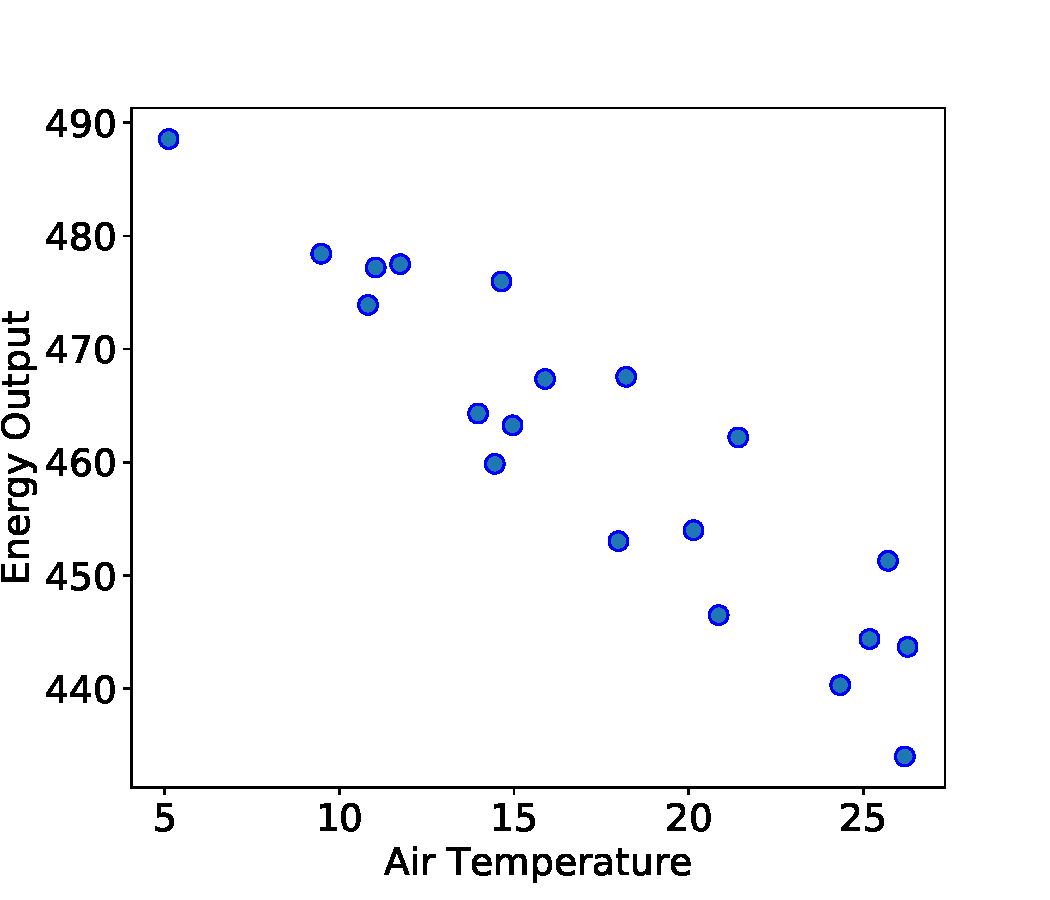
\includegraphics[
    width=\columnwidth,
    trim=0mm 0mm 10mm 10mm,
    clip=True]
    {univariate_scatter.pdf}
\end{figure}
\end{center}
}
\end{column}
\end{columns}

\end{frame}



\begin{frame}[t]
\frametitle{Univariate linear regression}

\vspace{-10mm}
\begin{columns}[t]
\begin{column}{0.55\textwidth}

\begin{itemize}

\only<1->{
\item Which fit to choose?
}
\only<2->{
\item With the linear model being fixed,
depends on the data and the \textit{loss function!}
}
\only<3->{
\item Mean square (L2) loss (MSE): 
\[
    Q(h, X^{\ell}) = \frac {1} {\ell} 
    \sum\limits_{i=1} ^{\ell} 
        (y_i - h(x_i))^2
\]
}

\end{itemize}

\end{column}
\begin{column}{0.45\textwidth}

\only<1->{
\begin{center}
\begin{figure}[t!]
    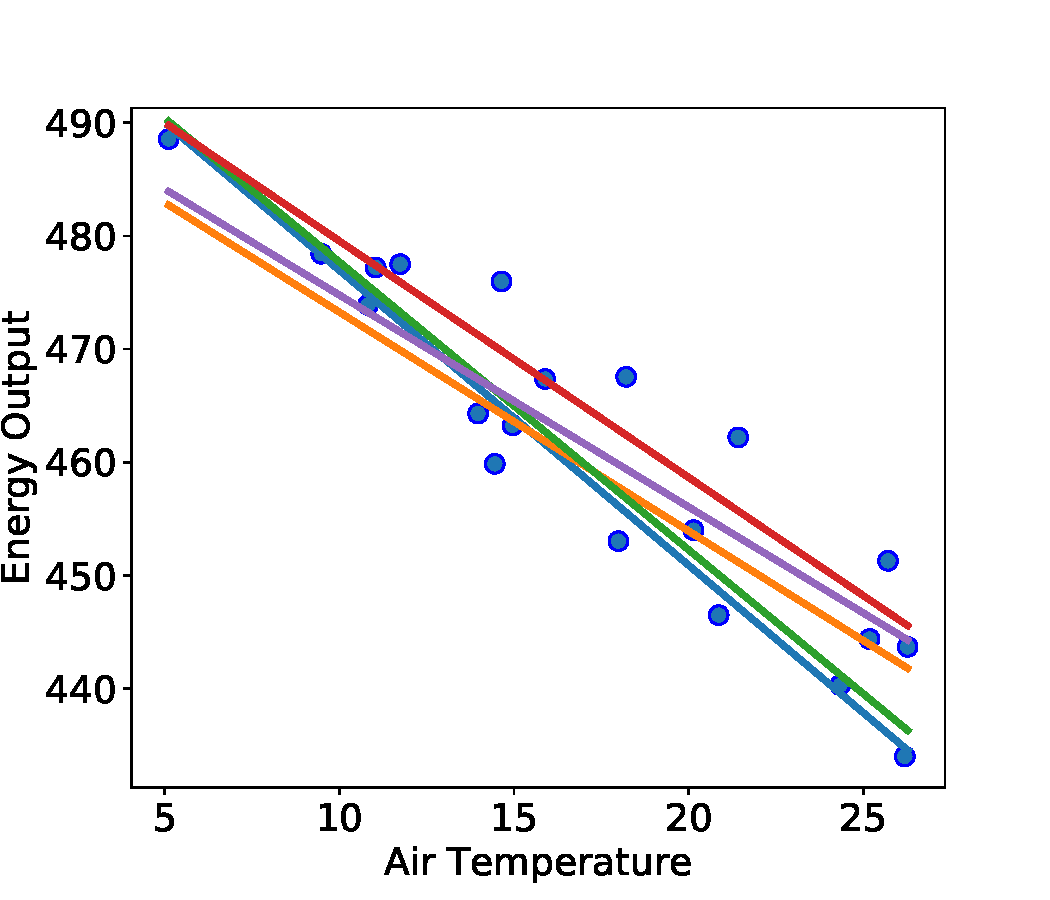
\includegraphics[
    width=\columnwidth,
    trim=0mm 0mm 10mm 10mm,
    clip=True]
    {univariate_scatter_fits.pdf}
\end{figure}
\end{center}
}
\end{column}
\end{columns}

\end{frame}



\begin{frame}
\frametitle{Some other evaluation metrics for regression}

\begin{itemize}

\item Mean square (L2) loss (MSE): 
$\mathrm{MSE}(h, X^{\ell}) = 
    \frac {1} {\ell} \sum\limits_{i=1} ^{\ell} (y_i - h(x_i))^2$

\pause
\item Root MSE: $\mathrm{RMSE}(h, X^{\ell}) =
\sqrt{\frac {1} {\ell} \sum\limits_{i=1} ^{\ell} (y_i - h(x_i))^2}$

\pause
\item Coefficient of determination:
$R^2 (h, X^{\ell}) = 1 -
\frac{\sum_{i=1}^{\ell} (y_i - h(x_i))^2}
{\sum_{i=1}^{\ell} (y_i - \mu_y)^2}$\\
with~$\mu_y = \frac{1}{\ell} \sum_{i=1}^{\ell} y_i$

\pause
\item Mean absolute error: 
$\mathrm{MAE}(h, X^{\ell}) =
    \frac {1} {\ell} \sum\limits_{i=1} ^{\ell} |y_i - h(x_i)|$

\end{itemize}

\end{frame}



\begin{frame}[t]
\frametitle{Univariate linear regression}

\vspace{-10mm}
\begin{columns}[t]
\begin{column}{0.55\textwidth}

\begin{itemize}

\only<1->{
\item With the loss fixed, the linear problem reduces to optimization: 
\[
\frac {1} {\ell} 
    \sum\limits_{i=1} ^{\ell} (y_i - w_1 x_i - w_0)^2
\to \min\limits_{(w_0, w_1) \in \mathbb{R}^2},
\]
}
% \[
% \frac {1} {\ell} \sum\limits_{i=1} ^{\ell} (y_i - h(x_i; \mathbf{w}))^2
% \to \min\limits_{\mathbf{w} \in \mathbb{R}^2}
% \]
% \item For the linear model
% yielding the system of equations
% \[
% \begin{cases}
% - \frac {1} {\ell} 
%     \sum\limits_{i=1} ^{\ell} 2 (y_i - w_1 x_i - w_0) = 0, \\
% - \frac {1} {\ell} 
%     \sum\limits_{i=1} ^{\ell} 2 (y_i - w_1 x_i - w_0)x_i = 0,
% \end{cases}
% \]
\only<2->{
to which an analytical solution is available
\begin{align*}
\widehat{w}_1 &= 
    \frac{\sum_{i=1}^{\ell} (x_i - \mu_x) (y_i - \mu_y)}
        {\sum_{i=1}^{\ell} (x_i - \mu_x)^2}, \\
\widehat{w}_0 &= \mu_y - \widehat{w}_1 \mu_x
\end{align*}
with $\mu_x = \frac{1}{\ell} \sum_{i=1}^{\ell} x_i,
\quad
\mu_y = \frac{1}{\ell} \sum_{i=1}^{\ell} y_i$
}
\end{itemize}

\end{column}
\begin{column}{0.45\textwidth}

\only<1->{
\begin{center}
\begin{figure}[t!]
    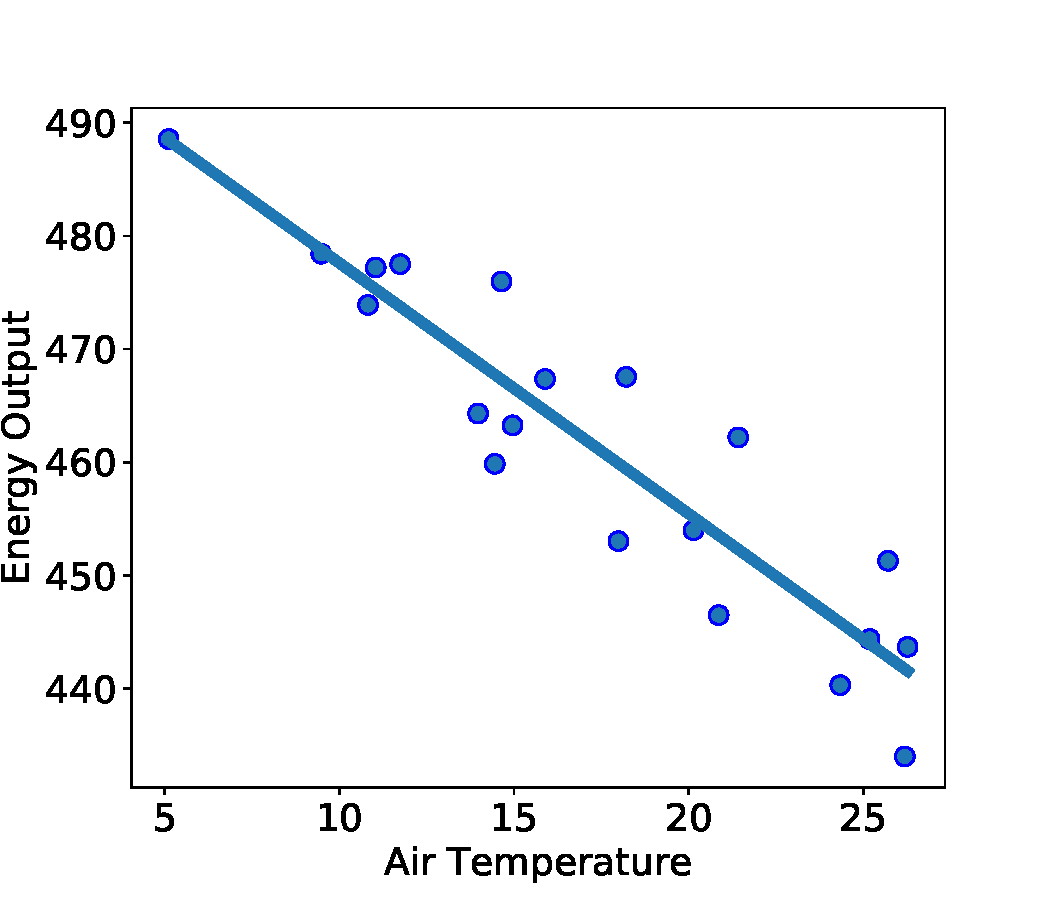
\includegraphics[
    width=\columnwidth,
    trim=0mm 0mm 10mm 10mm,
    clip=True]
    {univariate_scatter_mse_fit.pdf}
\end{figure}
\end{center}
}

\end{column}
\end{columns}

\end{frame}



\begin{frame}
\frametitle{Multivariate linear regression}

\begin{itemize}

\item Multiple features (regressors)
$\mathbf{x}_i = (x_{1i}, \ldots x_{d i})$
available for each $y_i$

\item The model: 
\vspace{-5mm}
\begin{align*}
y_1 &= w_1 x_{11} + \ldots w_d x_{d1} + \varepsilon_1, \\
y_2 &= w_1 x_{12} + \ldots w_d x_{d2} + \varepsilon_2, \\
& \ldots \\
y_{\ell} &= w_1 x_{1 \ell} + \ldots w_d x_{d \ell} + \varepsilon_{\ell}, 
\end{align*}
is often written in matrix-vector form as
\begin{align*}
\begin{bmatrix}
y_1 \\
% y_2 \\
\vdots \\
y_{\ell}
\end{bmatrix}
 = 
\begin{bmatrix}
    x_{11} & x_{12} & \dots  & x_{d1} \\
    % x_{12} & x_{22} & \dots  & x_{d2} \\
    \vdots & \vdots & \ddots & \vdots \\
    x_{1 \ell} & x_{2 \ell} & \dots  & x_{d \ell}
\end{bmatrix}
\begin{bmatrix}
w_1 \\
% w_2 \\
\vdots \\
w_d
\end{bmatrix}
+ 
\begin{bmatrix}
\varepsilon_1 \\
% \varepsilon_2 \\
\vdots \\
\varepsilon_{\ell}
\end{bmatrix}
\quad \longleftrightarrow \quad 
\bm{y} = \bm{X} \mathbf{w} + \bm{\varepsilon}
\end{align*}

\end{itemize}

\end{frame}



\begin{frame}
\frametitle{Multivariate linear regression: the solution}

\begin{itemize}

\item The problem: minimize MSE
\[
Q(h, X^{l}) = 
  \sum\limits_{i=1}^{\ell} 
  \big(y_i - \sum\limits_{k=1}^d w_k x_{ki}\big)^2
\equiv
\lVert \bm{y} - \bm{X} \mathbf{w}  \rVert^2 \to 
  \min_{\mathbf{w} \in \mathbb{R}^d}
\]

\pause
\item Solve analytically via computing the gradient
\[
\nabla_{\mathbf{w}} \lVert \bm{y} - \bm{X} \mathbf{w} \rVert^2
=
2 (\bm{y} - \bm{X}\mathbf{w})\bm{X} = 0
\]

\pause
\item The solution
\[
\mathbf{w}^* = ( \bm{X}^{\intercal} \bm{X} )^{-1} \bm{X}^{\intercal} \bm{y}
\]

\end{itemize}

\end{frame}



\section{Numerical and stochastic optimization at a glance}



\begin{frame}
\frametitle{A quick intro into the Numerical Optimization}

\begin{itemize}

\item Consider the \textcolor{Plum}{optimization problem}
in $\mathbb{R}^d$
\vspace{-5mm}
\[
f(\mathbf{x}) \to \min_{\mathbf{x} \in \mathbb{R}^d}
\qquad \qquad 
\mbox{(such as }
f(\mathbf{w}) \equiv 
\sum\limits_{i=1}^{\ell} 
  \Big(y_i - \sum\limits_{k=1}^d w_k x_{ki}\Big)^2
  \to \min\limits_{\mathbf{w} \in \mathbb{R}^d}\mbox{)}
\]
\end{itemize}

\pause
\vspace{-5mm}
\begin{columns}
\begin{column}{0.5\textwidth}
\begin{itemize}

\item In general, solved using the numerical methods
such as the \textcolor{Plum}{gradient descent}

\item \textcolor{Plum}{Gradients:} directions in $\mathbb{R}^d$
pointing towards steepest function increase
\[
\nabla_{\mathbf{x}} f(\mathbf{x}) \equiv 
\Big(
\frac{\partial f(\mathbf{x})}{\partial x_1},
\ldots,
\frac{\partial f(\mathbf{x})}{\partial x_d}
\Big)
\]

\begin{center}
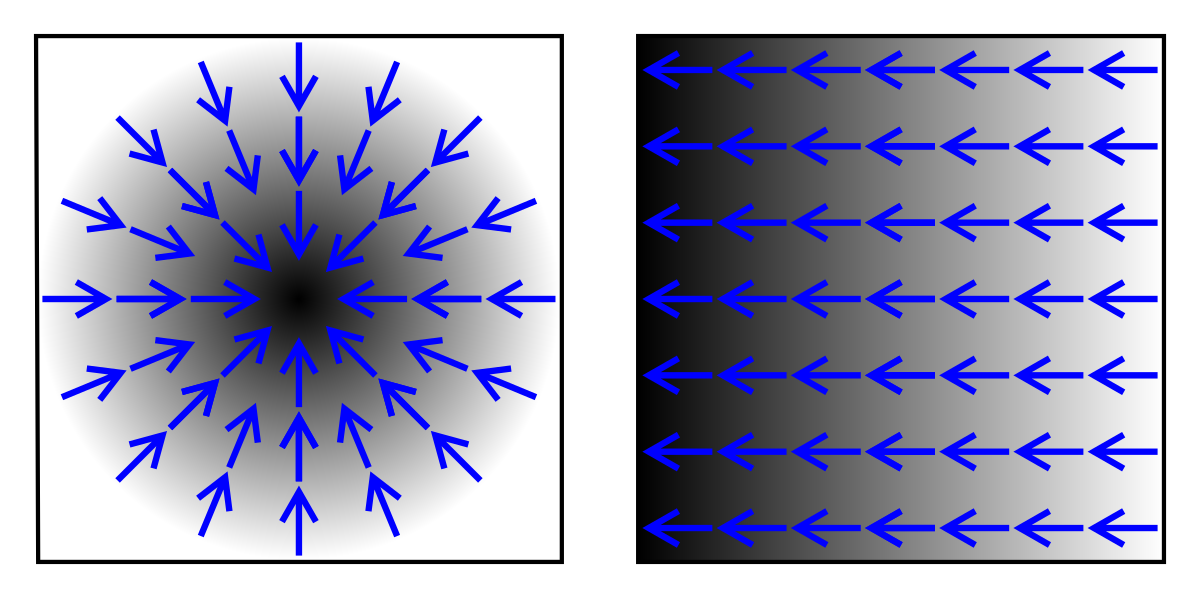
\includegraphics[width=0.5\columnwidth]{gradient_example.png}
\end{center}
\end{itemize}

\end{column}
\begin{column}{0.5\textwidth}  %%<--- here
    \begin{center}
     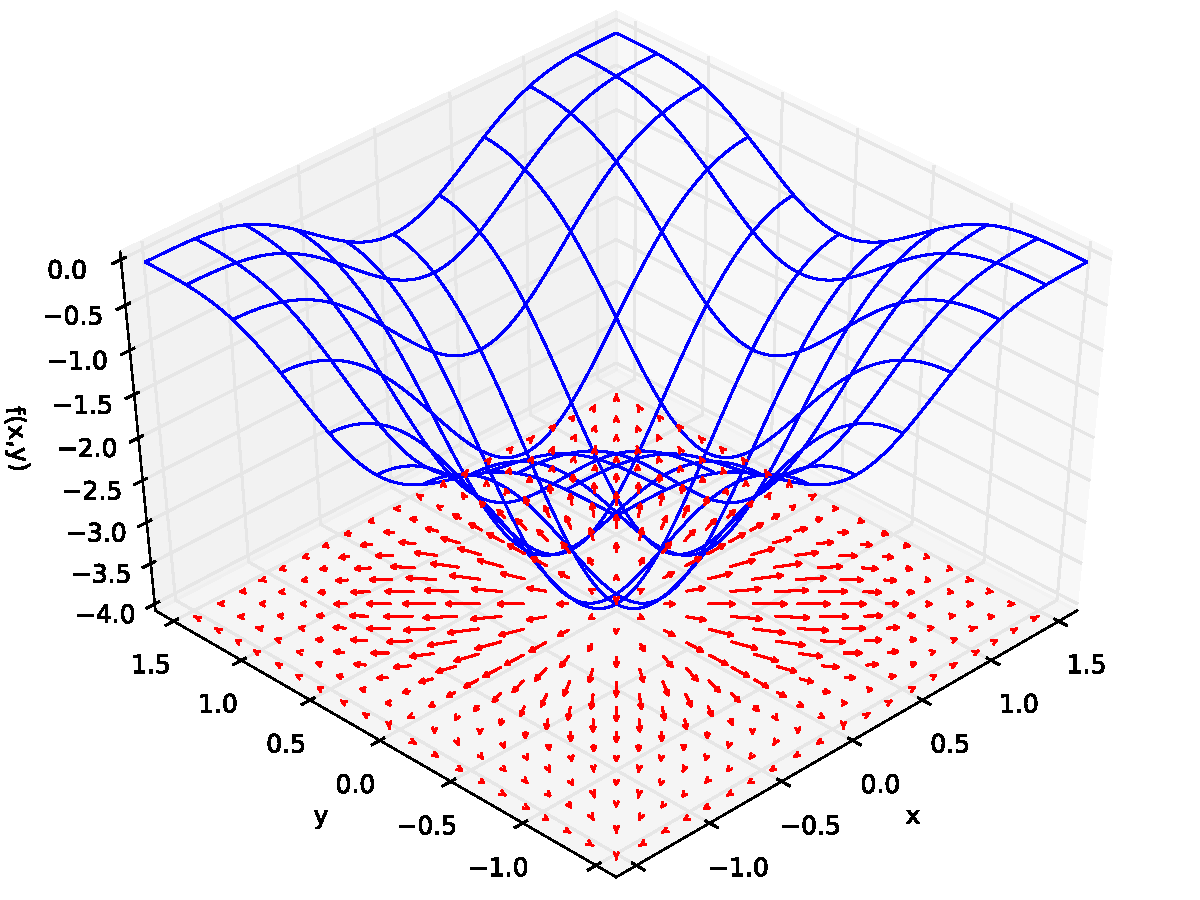
\includegraphics[width=0.9\columnwidth]{linregr-gradient-visual.pdf}
     \end{center}
\end{column}
\end{columns}

\end{frame}



\begin{frame}
\frametitle{The gradient descent algorithm}

\begin{itemize}

\item The gradient descent procedure iterates from $\mathbf{x}^{(0)}$ as
\[
\mathbf{x}^{(k)} \leftarrow
\mathbf{x}^{(k-1)} - \alpha_k \nabla_{\mathbf{x}} f(\mathbf{x}^{(k-1)})
\]
with $\alpha_k$ controlling the $k$th step size

\pause 
\item For smooth \textcolor{orange}{convex} functions with a single minimum $\mathbf{x}^*$,
$k$ steps of gradient descent achieve accuracy 
$f(\mathbf{x}^{(k)}) - f(\mathbf{x}^*) = \mathcal{O}(1/k)$

\begin{center}
  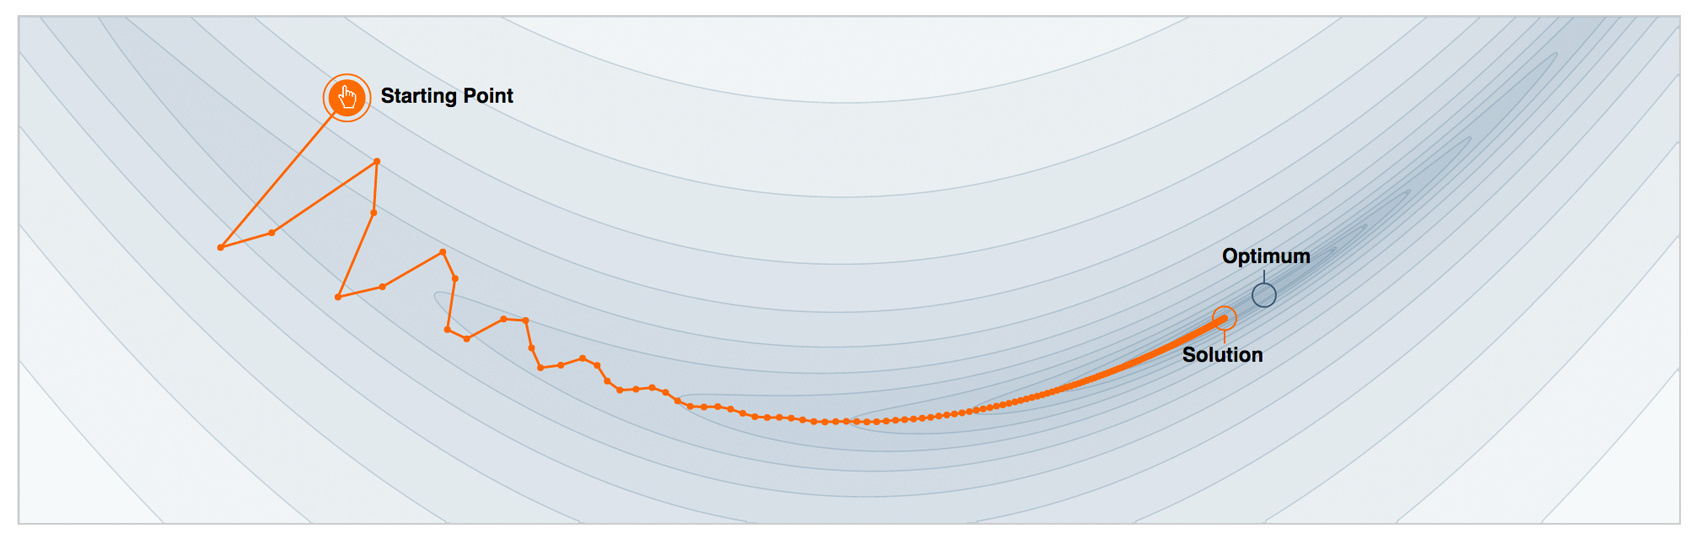
\includegraphics[width=0.8\columnwidth]{gradient_descent.png}
\end{center}

\end{itemize}

\end{frame}



\begin{frame}
\frametitle{The gradient descent with non-convex targets}

\begin{center}
  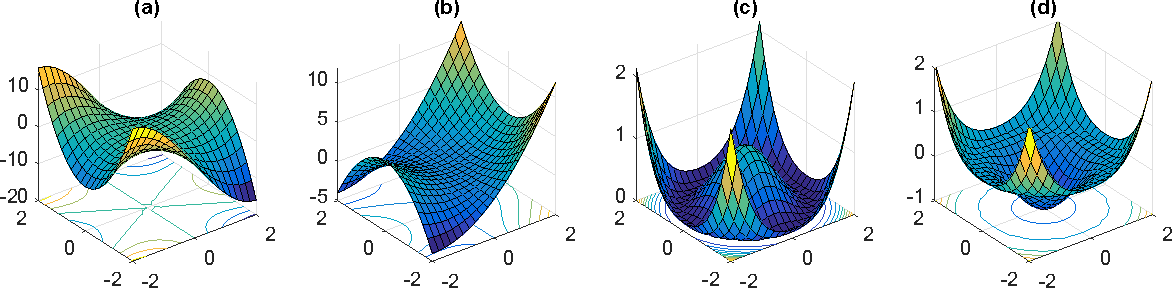
\includegraphics[width=1.\columnwidth]{nonconvex_functions.png}
\end{center}

\pause

\vspace{-2em}

\begin{columns}
\begin{column}{0.5\textwidth}

    \begin{itemize}

    \item Trajectories of gradient descent over \textcolor{orange}{non-convex functions}
    may (and will) not always end up in a single optimum

    \end{itemize}

\end{column}
\begin{column}{0.5\textwidth}  %%<--- here

\begin{center}
  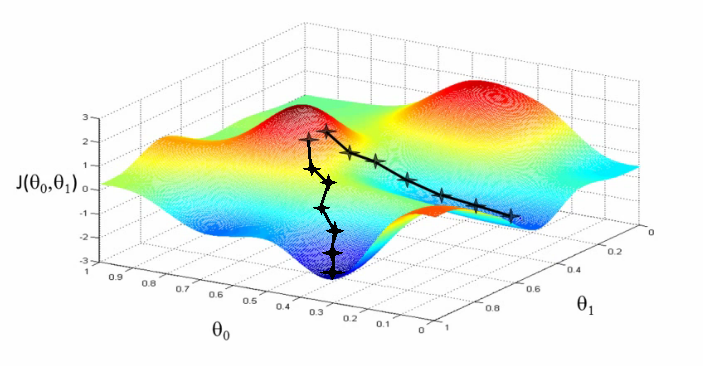
\includegraphics[width=1.\columnwidth]{nonconvex_sgd.png}  
\end{center}

\end{column}
\end{columns}

\end{frame}



% \begin{frame}
% \frametitle{The gradient descent with non-convex targets}

% \begin{center}
%   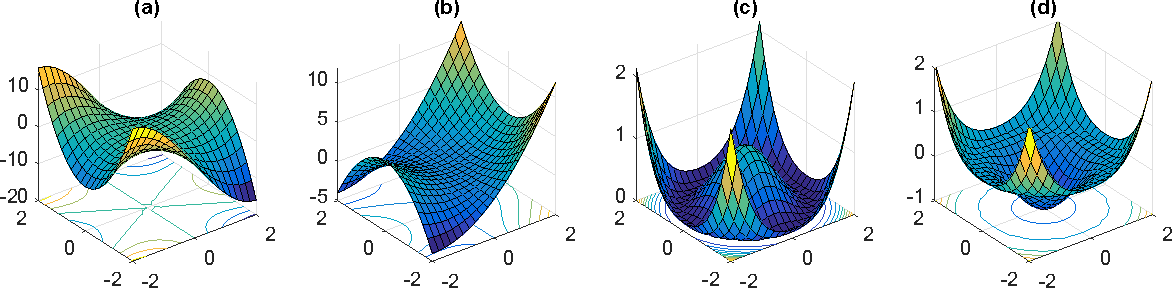
\includegraphics[width=1.\columnwidth]{nonconvex_functions.png}
% \end{center}

% \end{frame}



\begin{frame}
\frametitle{The stochastic gradient descent algorithm}

\begin{itemize}

\item Machine learning: many \textit{additive} targets
$f(\mathbf{w}) = \sum\limits_{i=1}^{\ell} f_i(\mathbf{w})$,\\
computationally inefficient for large $\ell$

\pause
\item Use subsamples for gradient \textit{estimation}:
the Stochastic Gradient Descent (SGD)
\begin{enumerate}
  % \Large
  \item $\mbox{Pick } i_k \in \{1, \ldots, \ell\} \mbox{ at random;}$
  \item Compute 
$\mathbf{w}^{(k)} \leftarrow
\mathbf{w}^{(k-1)} - \alpha_k
  \nabla_{\mathbf{w}} f_{i_k}(\mathbf{w}^{(k-1)})$
\end{enumerate}

\pause
\item For smooth convex functions with a single minimum $\mathbf{x}^*$,
$k$ steps of SGD achieve accuracy 
$f(\mathbf{w}^{(k)}) - f(\mathbf{w}^*) = \mathcal{O}(1/\sqrt{k})$

\pause
\item Batching, variance reduction, momentum hacks available
to improve the convergence rate to $\mathcal{O}(1/k)$

\end{itemize}

\end{frame}



\begin{frame}
\frametitle{Gradient descent VS stochastic gradient descent}

\begin{center}
  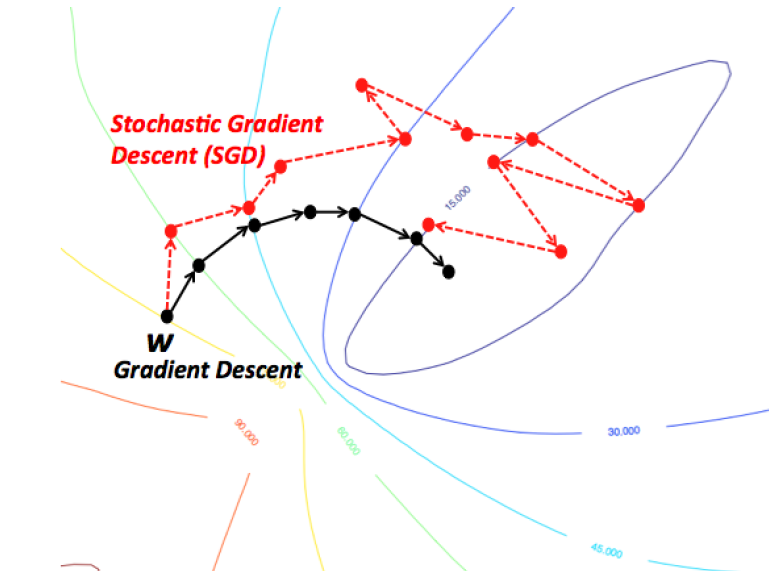
\includegraphics[width=0.7\columnwidth]
    {stochastic-vs-batch-gradient-descent.png}
\end{center}


\end{frame}



\begin{frame}
\frametitle{An example: SGD for multivariate linear regression}

\begin{columns}
\begin{column}{0.5\textwidth}

\begin{itemize}

\item Initialize with some $\mathbf{w}^{(0)}$

\item Gradient in $i_k$th object is
\[
\nabla_{\mathbf{x}} f_{i_k}(\mathbf{w}) = 
2 (y_{i_k} - \mathbf{x}_{i_k}^{\intercal}\mathbf{w})\mathbf{x}_{i_k}
\qquad (\in \mathbb{R}^d)
\]

\item Compute updates using SGD: 
$\mathbf{w}^{(k)} \leftarrow
\mathbf{w}^{(k-1)} - \alpha_k
  \nabla_{\mathbf{w}} f_{i_k}(\mathbf{w}^{(k-1)})$

\end{itemize}

\end{column}
\begin{column}{0.5\textwidth}  %%<--- here

\begin{center}
  \animategraphics[loop,autoplay,width=0.9\columnwidth]{12}{regressionfit/regressionfit-}{0}{14}
\end{center}

\end{column}
\end{columns}

\end{frame}



% \begin{frame}
% \frametitle{}

\section{Linear models for~classification}

% \end{frame}



\begin{frame}
\frametitle{Binary classification}

\begin{itemize}

\item An unknown distribution $D$
generates instances ($\mathbf{x}_1, \mathbf{x}_2, \ldots$)

\pause
\item An unknown function 
$f: \mathbb{X} \to \mathbb{Y}$ generates labels
($y_1, y_2, \ldots$) for them
such that $y_i = f(\mathbf{x}_i)$, and $y_i \in \{-1, +1\}$

\pause
\item {\bf Any examples of such functions? Implications?}

\end{itemize}

\pause

\begin{columns}
\begin{column}{0.4\columnwidth}
\begin{center}
  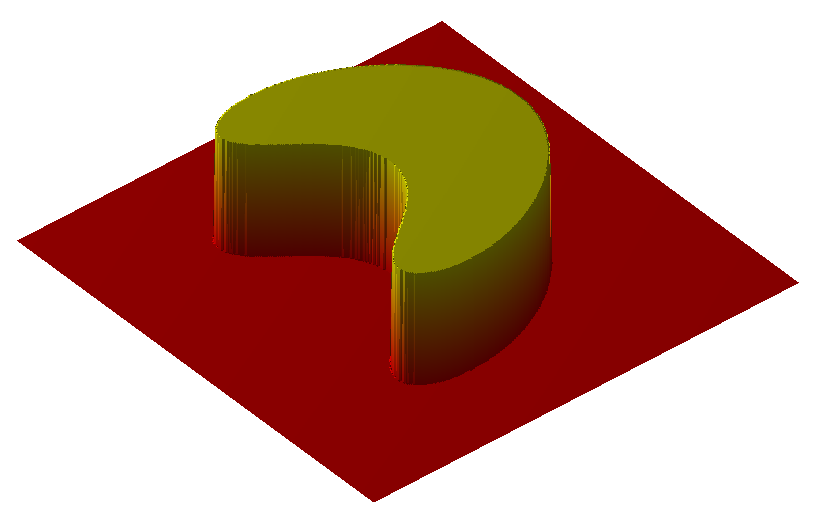
\includegraphics[
    width=\columnwidth,
    clip=True]
    {Indicator_function_illustration.png}
\end{center}
\end{column}
\begin{column}{0.6\columnwidth}
  There exist sets $A^{+}, A^{-}$
  such that
    $A^{+} \equiv \{i: \mathbf{x}_i \in D: y_i = +1\}$
  and   
    $A^{-} \equiv \{i: \mathbf{x}_i \in D: y_i = -1\}$
  with indicator functions $\chi_{A^{+}}(\cdot), \chi_{A^{-}}(\cdot)$
  (displayed on the left)
\end{column}
\end{columns}

\end{frame}



\begin{frame}
\frametitle{Binary classification}

\begin{itemize}

\item An unknown distribution $D$
generates instances ($\mathbf{x}_1, \mathbf{x}_2, \ldots$)

\item An unknown function 
$f: \mathbb{X} \to \mathbb{Y}$ generates labels
($y_1, y_2, \ldots$) for them
such that $y_i = f(\mathbf{x}_i)$, and $y_i \in \{-1, +1\}$

\item The classification problem:
choose a plausible hypothesis (\textcolor{orange}{classifier})
$h: \mathbb{X} \to \mathbb{Y}$
from the \textcolor{orange}{hypothesis space} $\mathbb{H}$

\pause
\item The error of the classifier $h$ is 
the probability (over $D$) that it will fail
\[
Q(h, D) = \mathrm{Pr}_{\mathbf{x} \sim D} 
  [f(\mathbf{x}) \neq h(\mathbf{x})]
\]
usually estimated by the \textcolor{Plum}{accuracy metric}
\[
    Q(h, X^{\ell}) = \frac {1} {\ell} 
    \sum\limits_{i=1} ^{\ell} 
        [f(\mathbf{x}_i) \neq h(\mathbf{x}_i)]
\]
\end{itemize}

\end{frame}



\begin{frame}
\frametitle{Linear models for classification}

\vspace{-10mm}
\begin{flushright}
  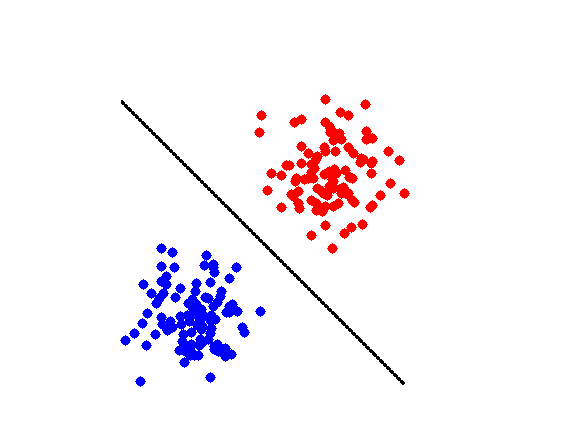
\includegraphics[
    width=0.25\columnwidth,
    trim=10mm 10mm 10mm 10mm,
    clip=True]
    {linear-classifier.png}
\end{flushright}

\vspace{-20mm}
\begin{itemize}

\item Linear model: 
$h(\mathbf{x}) = 
\mbox{sign} \big(\sum\limits_{i=1}^d w_i x_i + w_0\big) = 
\mbox{sign} \big(\mathbf{w}^{\intercal} \mathbf{x} + w_0\big)$

\pause
\item The learning problem is discrete
over $\mathbf{w} \in \mathbb{R}^d$:
\vspace{-2mm}
\[
    Q(h, X^{\ell}) = \frac {1} {\ell} 
    \sum\limits_{i=1} ^{\ell}     
        [\mbox{sign} (\mathbf{w}^{\intercal} \mathbf{x}_i)
           \neq h(\mathbf{x}_i)]
    \to \min\limits_{\mathbf{w} \in \mathbb{R}^d}
\vspace{-1mm}
\]
\pause
(\textcolor{red}{\textbf{cannot optimize using gradient descent}})

\begin{center}
  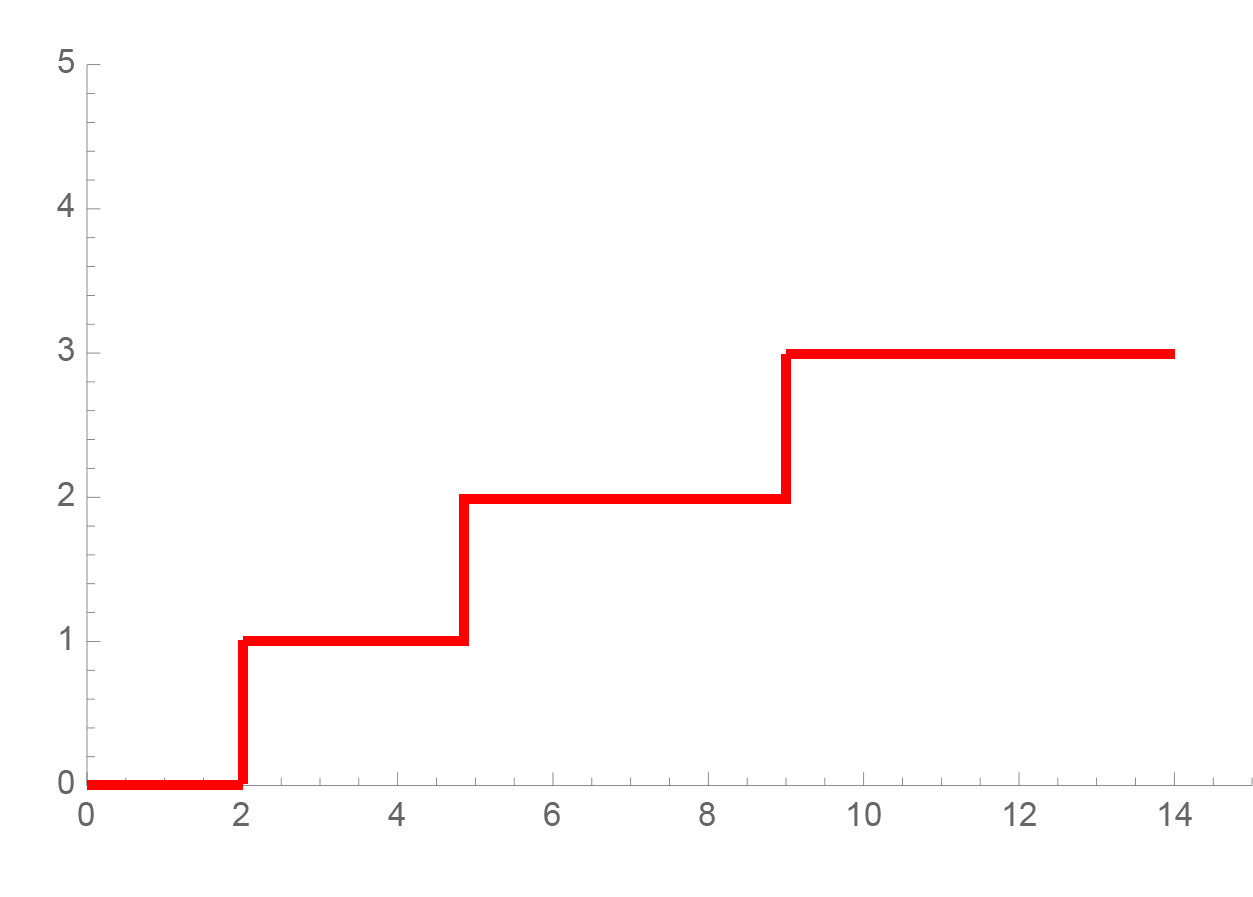
\includegraphics[
    width=0.5\columnwidth,
    trim=20mm 10mm 10mm 110mm,
    clip=True]
    {step_function.jpg}
\end{center}

\end{itemize}

\end{frame}



\begin{frame}
\frametitle{Linear models for classification}

\vspace{-10mm}
\begin{flushright}
  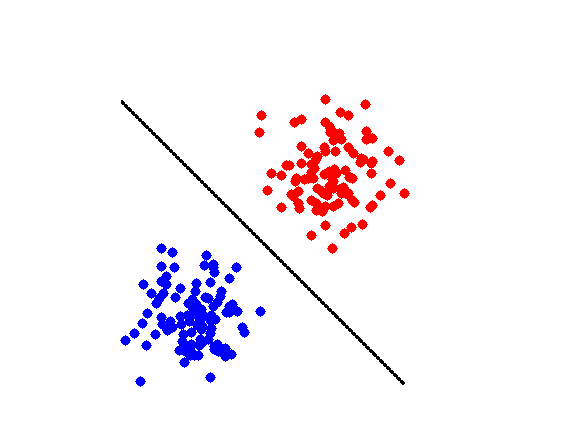
\includegraphics[
    width=0.25\columnwidth,
    trim=10mm 10mm 10mm 10mm,
    clip=True]
    {linear-classifier.png}
\end{flushright}

\vspace{-20mm}
\begin{itemize}

\item Linear model: 
$h(\mathbf{x}) = 
\mbox{sign} \big(\sum\limits_{i=1}^d w_i x_i + w_0\big) = 
\mbox{sign} \big(\mathbf{w}^{\intercal} \mathbf{x} + w_0\big)$

\item The learning problem is discrete
over $\mathbf{w} \in \mathbb{R}^d$:
\vspace{-2mm}
\[
    Q(h, X^{\ell}) = \frac {1} {\ell} 
    \sum\limits_{i=1} ^{\ell}     
        [\mbox{sign} (\mathbf{w}^{\intercal} \mathbf{x}_i)
           \neq h(\mathbf{x}_i)]
    \to \min\limits_{\mathbf{w} \in \mathbb{R}^d}
\vspace{-1mm}
\]

\item \textcolor{ForestGreen}{\textbf{The solution:}} optimize 
a 
\textcolor{orange}{\textit{differentiable upper bound}} for $Q(h, X^{\ell})$!

\pause
\item $Q(h, X^{\ell})$ can be written using 
$Q(h, X^{\ell}) = \frac {1} {\ell} \sum\limits_{i=1} ^{\ell} L(M_i)$\\
where $L(M_i) = [M_i < 0] 
\equiv [y_i \mathbf{w}^{\intercal} \mathbf{x}_i < 0]$

\item Upper-bounding $L(M)$ yields upper bounds for $Q(h, X^{\ell})$ 

\end{itemize}

\end{frame}





\begin{frame}
\frametitle{Linear models for classification: upper bounds}


\vspace{-2.5mm}
\begin{columns}
\begin{column}{0.4\textwidth}

Multiple approximations to accuracy
\begin{itemize}

\item $L_{\mbox{L}}(M) = \log(1 + e^{-M})$
\item $L_{\mbox{H}}(M) = \max(0, 1 - M)$
\item $L_{\mbox{P}}(M) = \max(0, -M)$
\item $L_{\mbox{E}}(M) = e^{-M}$
\item $L_{\mbox{S}}(M) = 2 / (1 + e^{M})$

\end{itemize}
and their respective optimization procedures
give rise to various learning algorithms

\end{column}
\begin{column}{0.6\textwidth}  %%<--- here
    \begin{center}
    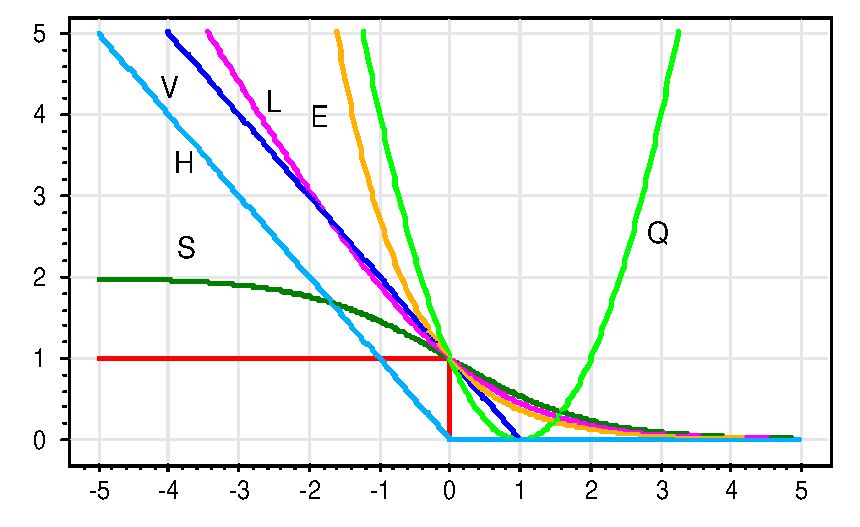
\includegraphics[width=\columnwidth]{threshold-approx-2.eps}
     \end{center}
\end{column}
\end{columns}

\end{frame}



\begin{frame}
\frametitle{The logistic regression model}

\begin{itemize}

  \item Training set $X^{\ell} = 
    \big\{(\mathbf{x}_i, y_i)\big\}_{i=1}^{\ell}$
    where $y_i \in \{-1, +1\}$

  \pause
  \item We seek an algorithm $h$ such that
  $h(\mathbf{x}) = \mathrm{P}(y = +1 | \mathbf{x})$
  (\textcolor{Plum}{model probability!})

  \pause
  \item A probability that an instance $(\mathbf{x}_i, y_i)$
  is encountered in $X^{\ell}$
  \[
  h(\mathbf{x}_i)^{[y_i = +1]} + (1 - h(\mathbf{x}_i))^{[y_i = -1]}
  \]

  \pause
  \item Entire $X^{\ell}$ likelihood:
  \vspace{-2mm}
  \[
  L(X^{\ell}) = \prod\limits_{i=1}^{\ell}
    h(\mathbf{x}_i)^{[y_i = +1]} + (1 - h(\mathbf{x}_i))^{[y_i = -1]}
  \vspace{-2mm}
  \]
  \pause
  is often written via \textcolor{orange}{log-likelihood}
  (of which the negative is \textcolor{orange}{log-loss})
  \vspace{-2mm}
  \[
  \log L(X^{\ell}) = \sum\limits_{i=1}^{\ell}
    [y_i = +1] \log h(\mathbf{x}_i) + 
    [y_i = -1] \log (1 - h(\mathbf{x}_i))
  \]

\end{itemize}

\end{frame}



\begin{frame}
\frametitle{The logistic regression model}

% 
\vspace{-2.5mm}
\begin{columns}
\begin{column}{0.55\textwidth}

\begin{itemize}

  \item The choice of $h$: sigmoid function
  \[
  h(\mathbf{x}) = \sigma(\mathbf{w}^{\intercal} \mathbf{x})
  \]
  where $\sigma(x) \in [0, 1]$

  \item Typical choice: the logistic function
  \[
  \sigma(\mathbf{w}^{\intercal} \mathbf{x}) = 
  \frac{1} {1 + \exp(-\mathbf{w}^{\intercal} \mathbf{x})}
  \]

  \item Plugging the logistic function into
  the loss yields an approximation of accuracy
  \vspace{-2mm}
  \[
  \sum\limits_{i=1}^{\ell}
    (1 + \exp(\mathbf{w}^{\intercal} \mathbf{x}))
    \to \min\limits_{\mathbf{w} \in \mathbb{R}^d}
  \]

\end{itemize}

\end{column}
\begin{column}{0.45\textwidth}  %%<--- here
    \begin{center}
    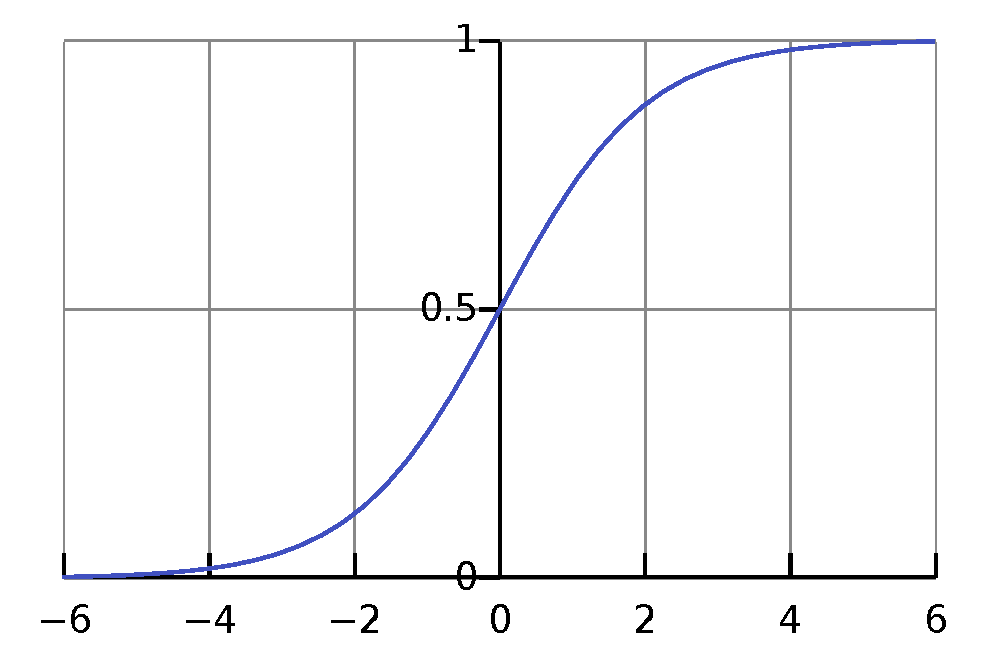
\includegraphics[width=\columnwidth]{linregr-logistic-func.pdf}
     \end{center}
\end{column}
\end{columns}

\end{frame}



\begin{frame}
\frametitle{The logistic regression model}

\begin{center}
    % \fbox{
    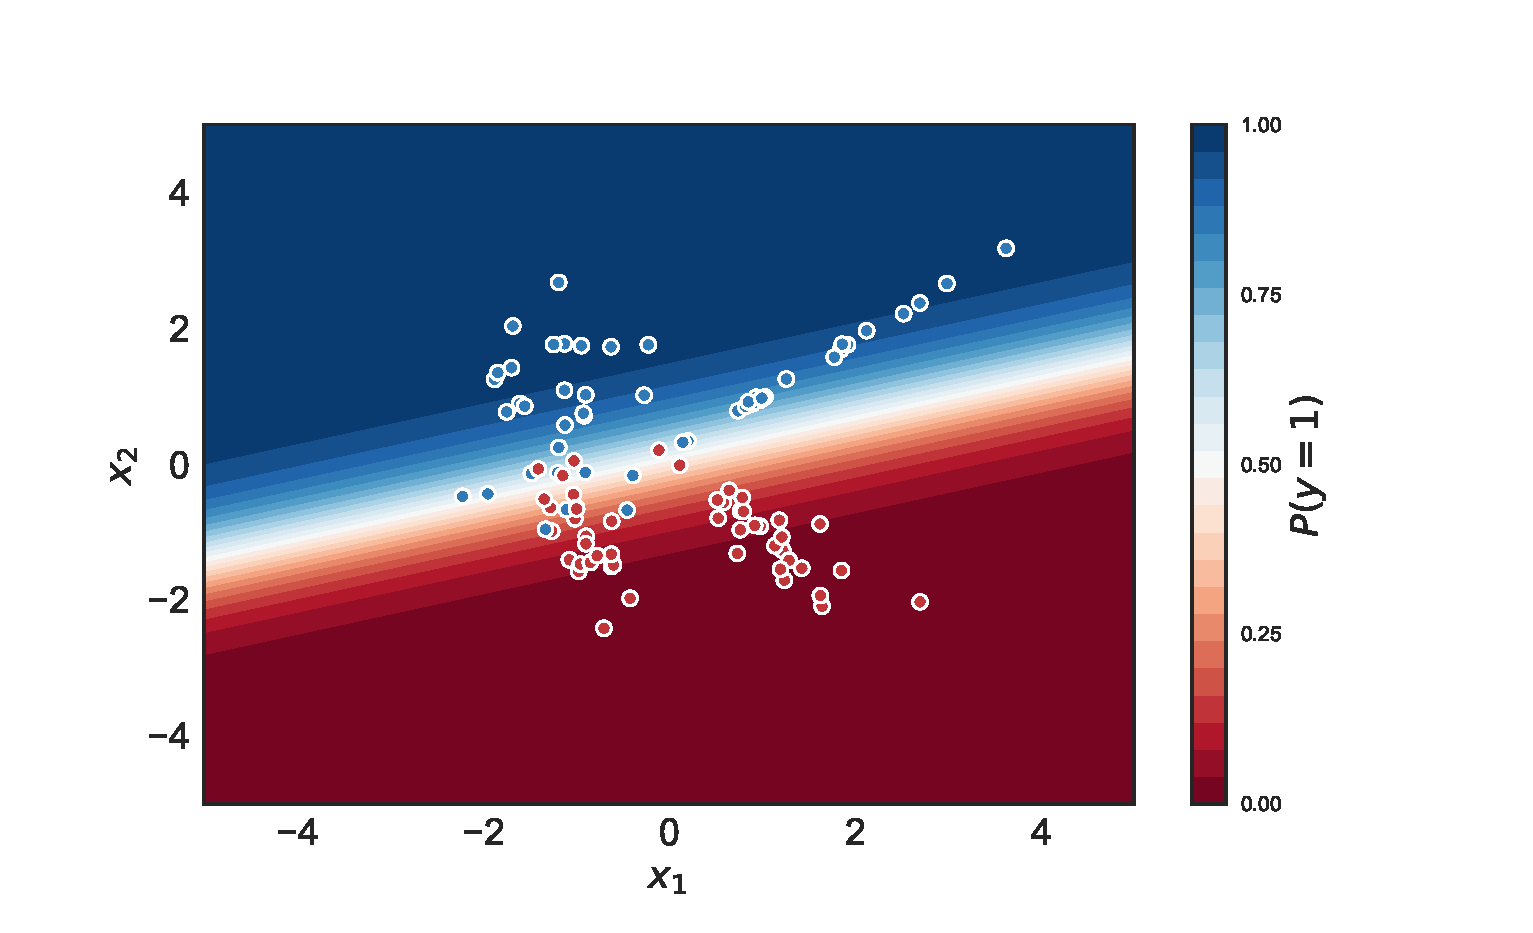
\includegraphics[
    width=0.75\columnwidth,
    trim=10mm 5mm 25mm 15mm,
    clip=True]
        {logistic-regression-boundary.eps}
    % }
\end{center}

\end{frame}



% \begin{frame}
% \frametitle{}

\section{Figures of merits}


% \end{frame}


\begin{frame}
\frametitle{Classification quality evaluation: accuracy}

\begin{itemize}
\item Given a labeled sample $X^{\ell} = 
    \big\{(\mathbf{x}_i, y_i)\big\}_{i=1}^{\ell}$,
    $y_i \in \{-1, +1\}$,
and some candidate~$h$, \textbf{\textcolor{Plum}{how well
does $h$ perform on $X^\ell$?}}

\pause
\item Let the thresholded decision rule be $a(x) = [h(x) > t]$
($t$: hyperparameter)

\pause
\item Obvious choice: \textcolor{orange}{accuracy}
\[
    \text{accuracy}(a, X^\ell)
    =
    \frac{1}{\ell}
    \sum\limits_{i = 1}^{\ell} [a(\mathbf{x}_i) = y_i]
\]

\end{itemize}

\begin{columns}
    \vspace{-5mm}
    \begin{column}{0.75\textwidth}
    \begin{itemize}
        \item Example: Higgs challenge -- 
        selection of the \textcolor{Plum}{interesting signal} 
        $H \to \tau \tau$ 
        decay against the \textcolor{Plum}{already known backround}

        \item 164,333 background, 85,667 signal events (66\% background)
    \end{itemize}
    \end{column}
    \begin{column}{0.25\textwidth}
    
\includegraphics[width=0.9\columnwidth]{higgs_challenge.png}
    \end{column}
\end{columns}

\end{frame}



\begin{frame}
\frametitle{Classification quality evaluation: confusion matrix}

\begin{table}[t]
    \centering
    \begin{tabular}{|l|c|c|}
        \hline
        & Label $y = 1$ & Label $y = -1$ \\ \hline
        Decision $a(x) = 1$ & True Positive (TP) & False Positive (FP) \\ \hline
        Decision $a(x) = -1$ & False negative (FN) & True Negative (TN) \\ \hline
    \end{tabular}
\end{table}

\begin{itemize}
    \pause
    \item \textcolor{orange}{Rates} are often more informative:
    \begin{align*}
    \text{False Positive Rate aka FPR}
    =
    \frac{
        \text{FP}
    }{
        \text{FP} + \text{TN}
    }, \\
    \text{True Positive Rate aka TPR}
    =
    \frac{
        \text{TP}
    }{
        \text{TP} + \text{FN}
    },
\end{align*}


\pause
\item While accuracy can be expressed, too
\[
    \text{accuracy}
    =
    \frac{\text{TP} + \text{TN}}{\text{TP} + \text{FP} + \text{FN} + \text{TN}}
\]

\end{itemize}

\end{frame}



\begin{frame}
\frametitle{Classification quality: the receiver operating curve}

\begin{columns}
\begin{column}{0.6\textwidth}
    \begin{itemize}
        \item Often $h(\mathbf{x})$ is more
        valuable than its thresholded
        version $a(x) = [h(x) > t]$

        \pause
        \item Consider two-dimensional
        space with coordinates (TPR($t$), FPR($t$)),
        corresponding to various choices of the threshold $t$

        \pause 
        \item The plot TPR($t$) vs. FPR($t$) is called the
        \textcolor{orange}{receiver operating
        characteristic} (ROC) curve

        \pause
        \item Area under curve (ROC-AUC) 
        reflects classification quality
    \end{itemize}
\end{column}

\begin{column}{0.4\textwidth}
    \begin{center}
        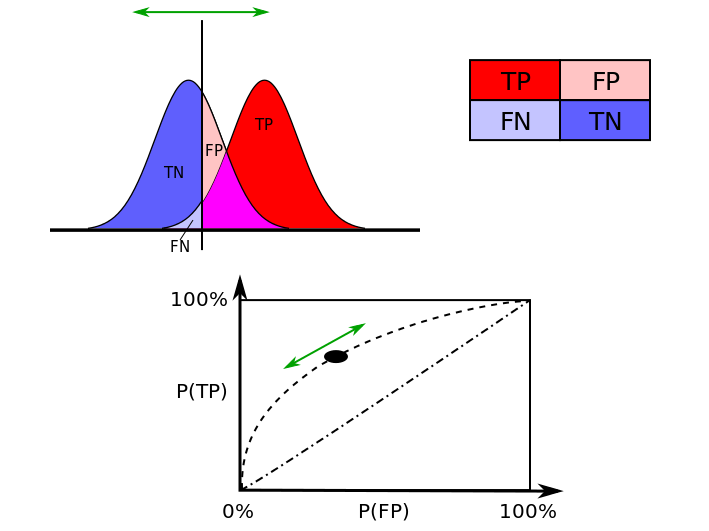
\includegraphics[
        width=1.1\columnwidth,
        trim=10mm 2mm 10mm 6mm,
        clip=False]
        {roc_curve.png}

        \footnotesize{\textcolor{gray}{Source: Wikipedia}}
    \end{center}
\end{column}
\end{columns}

\end{frame}



\begin{frame}
\frametitle{Classification quality: imbalanced data}

\begin{itemize}
    \item Recall the Higgs: 164,333 background vs.
    85,667 signal events (66\% background)

    \pause
    \item TPR($t$) vs. FPR($t$) / ROC
    is \textcolor{red}{bad for imbalanced data:}
    for $\ell = 1000$,\\
    $n_{-} = 950$ (high background noise),
    $n_{+} = 50$ (low signal),\\
    a trivial rule $h(\mathbf{x}) = -1$ (``treat everything as background'')
    would yield:
    \begin{itemize}
        \pause
        \item $\text{accuracy}(a, X^\ell) = 0.95$ (\textcolor{red}{bad})

        \pause
        \item $\text{TPR}(a, X^\ell) = 0.$ (\textcolor{SpringGreen}{OK})

        \pause
        \item $\text{FPR}(a, X^\ell) = 0.$ (\textcolor{red}{bad})
    \end{itemize}

    \pause
    \item Criteria better suited for imbalanced problems:
    \begin{align*}
        &\text{precision}
        =
        \frac{
            \text{TP}
        }{
            \text{TP} + \text{FP}
        }, \qquad
        \text{recall}
        =
        \frac{
            \text{TP}
        }{
            \text{TP} + \text{FN}
        }
    \end{align*}

\end{itemize}

\end{frame}



\begin{frame}[t]
\frametitle{Classification quality: imbalanced data}

\begin{columns}
\begin{column}{0.5\textwidth}
    \begin{center}
        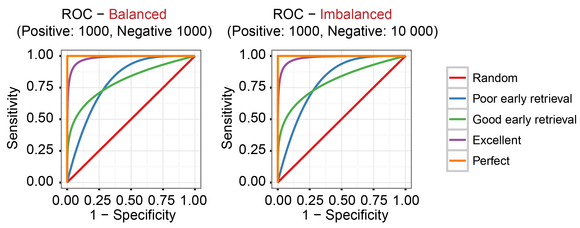
\includegraphics[
        width=1.0\columnwidth]
        {roc-balanced-imbalanced.png}

        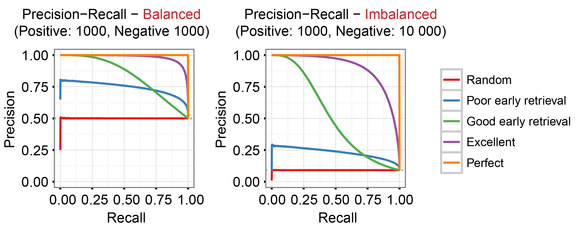
\includegraphics[
        width=1.\columnwidth]
        {precision-recall-balanced-imbalanced.png}

        \footnotesize{\textcolor{gray}{Source: classeval.wordpress.com}}
    \end{center}
\end{column}
\begin{column}{0.5\textwidth}
    \begin{itemize}

        \item The plot recall vs. precision is called the
        \textcolor{orange}{precision-recall} (PR) curve

        \pause
        \item Recall($t$) vs. Precision($t$)
        is \textcolor{ForestGreen}{good for imbalanced data:}
        for $\ell = 1000$,\\
        $n_{-} = 950$ (high background noise),
        $n_{+} = 50$ (low signal),\\
        a trivial rule $h(\mathbf{x}) = -1$
        would yield:
        
        \pause
        \begin{itemize}
            \item $\text{Recall}(a, X^\ell) = 0.$ (\textcolor{ForestGreen}{OK})

            \item $\text{Precision}(a, X^\ell) = 0.$ (\textcolor{ForestGreen}{OK})
        \end{itemize}

    \end{itemize}
\end{column}

\end{columns}

\end{frame}



% \begin{frame}
% \frametitle{}

\section{Overfitting:~how~to~fool the~linear~regression}

% \end{frame}



\begin{frame}
\frametitle{Generalization and overfitting}

\begin{itemize}
  \item Training set memorization:
  for seen $(\mathbf{x}, y) \in X^{\ell}$, $h(\mathbf{x}) = y$

  \pause
  \item \textcolor{orange}{Generalization:} 
   equally good performance
  on both new and seen instances

  \pause
  \item How to assess model's generalization ability?

  \pause
  \item Consider an example: 

  \begin{itemize}
    % \Large
    \item $y = \cos (1.5 \pi x) + \mathcal{N}(0, 0.01)$, 
    $x \sim \mathrm{Uniform}[0, 1]$

    \item Features: $\{x\}$, $\{x, x^2, x^3, x^4\}$,
    $\{x, \ldots, x^{15}\}$

    \item The model is linear w.\,r.\,t. features:
    $f(\mathbf{x}) = \mathbf{w}^{\intercal} \phi(\mathbf{x})$
  \end{itemize}

  \pause
  \item How well do the regression models perform?

\end{itemize}

\end{frame}



\begin{frame}
\frametitle{Polynomial fits of different degrees}

\begin{center}
    \includegraphics[
    width=\columnwidth,
    trim=30mm 0 30mm 0,
    clip=True]
    {underfitting_overfitting.eps}
\end{center}

\end{frame}



% \begin{frame}
% \frametitle{The notion of model complexity}



% \end{frame}



\begin{frame}
\frametitle{Model validation and selection}

\begin{itemize}

  \item We have free parameters in models:
  \begin{itemize}
    \normalsize
    \pause
    \item polynomial degree $d$, 
    subset of features in multivariate regression, 
    kernel width in kernel density estimates, \ldots
  \end{itemize}

  \pause
  \item \textcolor{Plum}{\textbf{Model selection:}} how to select optimal
  hyperparameters for a given classification problem?

  \pause
  \item \textcolor{orange}{\textbf{Validation:}} how to estimate true model performance?

  \pause
  \item Can we use entire dataset to fit the model?

  \pause
  \item \textcolor{Plum}{\textit{Yes, but}} we will likely get overly optimistic performance estimate

  \pause
  \item \textcolor{ForestGreen}{\textbf{The solution:}} rely on held-out data to assess model performance

\end{itemize}

\end{frame}



\begin{frame}
\frametitle{Assessing generalization ability: train/validation}

\begin{columns}
\begin{column}{0.6\textwidth}
    
\begin{itemize}
  \item Split training set into two subsets:
  \[
  X^{\ell} = X^{\ell}_{\text{TRAIN}} \cup X^{\ell}_{\text{VAL}}
  \]

  \pause
  \item Train a model $h$ on $X^{\ell}_{\text{TRAIN}}$
    
  \pause
  \item Evaluate model $h$ on $X^{\ell}_{\text{VAL}}$

  \pause
  \item Assess quality using $Q(h, X^{\ell}_{\text{VAL}})$

  \pause
  \item \textcolor{BrickRed}{\textbf{Data-hungry:}} 
  can we afford the
  "luxury" of setting aside a portion of the data for testing?

\pause
  \item \textcolor{BrickRed}{\textbf{May be imprecise:}}
  the holdout estimate of error rate will be misleading
  if we happen to get an "unfortunate" split

\end{itemize}
\end{column}

\begin{column}{0.4\textwidth}
    \begin{center}
    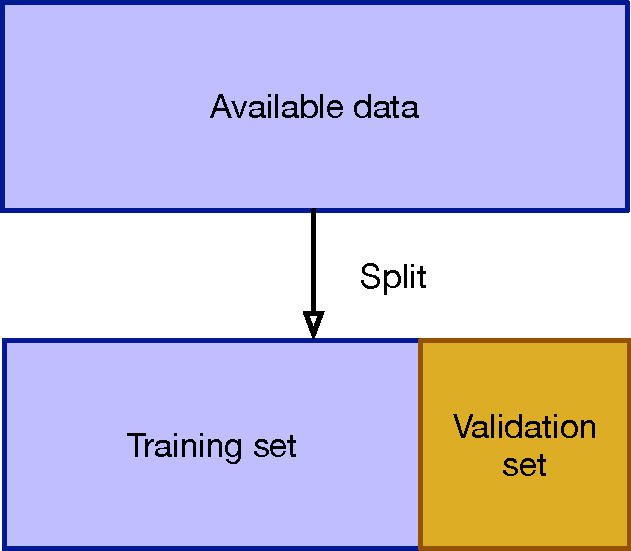
\includegraphics[
    height=0.8\textwidth]
    {cross-validation.pdf}
    \end{center}
\end{column}
\end{columns}

\end{frame}



\begin{frame}
\frametitle{Assessing generalization ability: cross-validation}

\begin{columns}
\begin{column}{0.6\textwidth}
    

\begin{itemize}
  \item Split training set into subsets of equal size $X^{\ell} = 
    X^{\ell}_{1} \cup \ldots \cup X^{\ell}_{K}$

  \pause
  \item Train $K$ models $h_1, \ldots, h_K$
  where each model~$h_k$ is trained on all subsets
  \textcolor{orange}{\textbf{but}} $X^{\ell}_k$
    
  \pause
  \item Assess quality using \\
  $\mathrm{CV} = \frac 1 K \sum\limits_{k=1}^K Q(h_k, X^{\ell}_k)$
  ($K$-fold)

  \pause
  \item Leave-one-out cross-validation:
    $X^{\ell}_k = \{(\mathbf{x}_k, y_k)\}$
    (yes, train $\ell$ models!)

\end{itemize}

\end{column}

\begin{column}{0.4\textwidth}

\begin{center}
    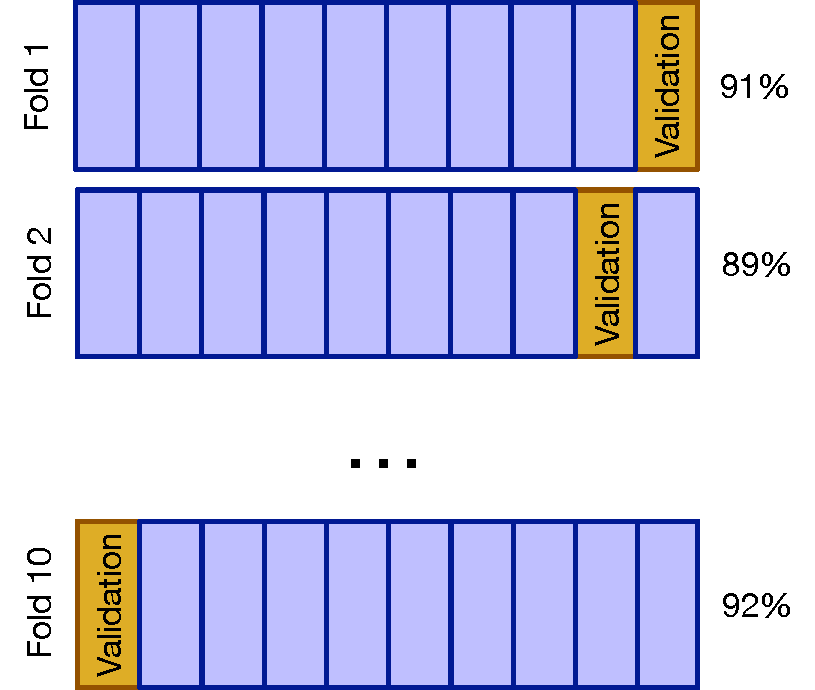
\includegraphics[
    height=0.9\textwidth]
    {cross-validation-folds.pdf}
\end{center}
\end{column}
\end{columns}

\end{frame}



% \begin{frame}
% \frametitle{10-fold cross-validation}


% \end{frame}



\begin{frame}
\frametitle{Cross-validation method: drawbacks}

\[
\mathrm{CV} = \frac 1 K \sum\limits_{k=1}^K Q(h_k, X^{\ell}_k)
\]

Many folds:
\begin{itemize}
  \item \textcolor{ForestGreen}{\textbf{Small bias:}} the estimator will be very accurate
  \item \textcolor{BrickRed}{\textbf{Large variance:}} due to small split sizes
  \item \textcolor{BrickRed}{\textbf{Costly:}} many experiments, large computational time 
\end{itemize}

\pause
Few folds:
\begin{itemize}
  \item \textcolor{ForestGreen}{\textbf{Cheap, computationally effective:}} few experiments
  \item \textcolor{ForestGreen}{\textbf{Small variance:}} average over many samples
  \item \textcolor{BrickRed}{\textbf{Large bias:}} estimated error rate conservative
  or smaller than the true error rate
\end{itemize}

\end{frame}





% \begin{frame}
% \frametitle{Assessing generalization ability: cross-validation}


% \begin{itemize}
%   \item Split training set into subsets of equal size $X^{\ell} = 
%     X^{\ell}_{1} \cup \ldots \cup X^{\ell}_{K}$

%   \pause
%   \item Train $K$ models $h_1, \ldots, h_K$
%   where each model $h_k$ is trained on all subsets
%   but $X^{\ell}_k$
    
%   \pause
%   \item Assess quality using 
%   $\mathrm{CV} = \frac 1 K \sum\limits_{k=1}^K Q(h_k, X^{\ell}_k)$
%   ($K$-fold)

%   \pause
%   \item Leave-one-out cross-validation:
%     $X^{\ell}_k = \{(\mathbf{x}_k, y_k)\}$

% \end{itemize}

% \end{frame}



% \begin{frame}
% \frametitle{Preventing overfitting}


% \end{frame}




% \begin{frame}
% \frametitle{}

\section{Regularization}

% \end{frame}



\begin{frame}
\frametitle{Ad-hoc regularization: motivation}

\begin{itemize}
  \item Consider the multivariate linear regression problem
  with $\bm{X} \in \RR^{d \times d}$
  \[
    \lVert \bm{y} - \bm{X} \mathbf{w}  \rVert^2 \to 
    \min_{\mathbf{w} \in \mathbb{R}^d}
  \]

  \pause
  \item Analytic solution involves 
  computing the
  product $\bm{R} =
  ( \bm{X}^{\intercal} \bm{X} )^{-1} \bm{X}^{\intercal}$

  \pause
  \item If $\bm{X} = \mbox{diag}(\lambda_1, \ldots, \lambda_d)$
    with $\lambda_1 > \lambda_2 > \ldots > \lambda_d \to 0$\\
    (meaning we're in eigenbasis of $\bm{X}$) then
  \begin{align*}
    \bm{R} &= ( \bm{X}^{\intercal} \bm{X} )^{-1} \bm{X}^{\intercal} = \\
    &= 
    \big(\mbox{diag}(\lambda_1, \ldots, \lambda_d)
    \mbox{diag}(\lambda_1, \ldots, \lambda_d)\big)^{-1}
    \mbox{diag}(\lambda_1, \ldots, \lambda_d) = \\
    &= \mbox{diag}\Big(\frac {1} {\lambda_1}, 
      \ldots, \frac {1} {\lambda_d}\Big),
      \quad
      \mbox{leading to huge diagonal values in $\bm{R}$ }
  \end{align*}

\end{itemize}

\end{frame}



\begin{frame}
\frametitle{Ad-hoc regularization: L2}

\begin{itemize}
  \item \textbf{Regularization:}
    replace \textcolor{orange}{fit} 
    with \textcolor{Fuchsia}{fit + penalty} as in 
    \[
    Q(\mathbf{w}) \to 
      Q_{\alpha}(\mathbf{w}) = Q(\mathbf{w}) + \alpha R(\mathbf{w})
    \]

  \pause
  \item $R(\mathbf{w})$ is called the \textit{regularizer},
  $\alpha > 0$ -- the \textit{regularization constant}


  \pause
  \item \textit{Regularized} multivariate linear regression problem
  \[
    \lVert \bm{y} - \bm{X} \mathbf{w}  \rVert^2 
    +
    \alpha \lVert \mathbf{w} \rVert^2_2
    \to 
    \min_{\mathbf{w} \in \mathbb{R}^d}
  \]

  \pause
  \item \textit{Regularized} analytic solution
  available
  \[
  \mathbf{w}^* =
  ( \bm{X}^{\intercal} \bm{X} + \alpha \bm{I})^{-1}
  \bm{X}^{\intercal} \bm{y}
  \]

\end{itemize}

\end{frame}



\begin{frame}
\frametitle{Why L2 regularization works}

\begin{itemize}
  \item Analytic solution: compute the regularized operator
  \[
  \bm{R} =
  ( \bm{X}^{\intercal} \bm{X} + \alpha \bm{I})^{-1} \bm{X}^{\intercal}
  \]

  \pause
  \item If $\bm{X} = \mbox{diag}(\lambda_1, \ldots, \lambda_d)$
    with $\lambda_1 > \lambda_2 > \ldots > \lambda_d \to 0$\\
    (meaning we're in eigenbasis of $\bm{X}$) then
    % \large
  \begin{align*}
    \bm{R} &= ( \bm{X}^{\intercal} \bm{X}  + \alpha \bm{I})^{-1}
      \bm{X}^{\intercal} = \\
    &= 
    \big(\mbox{diag}(\lambda_1, \ldots, \lambda_d)
    \mbox{diag}(\lambda_1, \ldots, \lambda_d)
    +
    \mbox{diag}(\alpha, \ldots, \alpha)
    \big)^{-1}
    \mbox{diag}(\lambda_1, \ldots, \lambda_d) = \\
    &= \mbox{diag}\Big(\frac {\lambda_1} {\lambda^2_1 + \alpha}, 
      \ldots, \frac {\lambda_d} {\lambda^2_d + \alpha}\Big),
  \end{align*}
    smoothing diagonal values in $\bm{R}$ 

\end{itemize}

\end{frame}



\begin{frame}
\frametitle{More regularizers!}

\begin{itemize}

  \item \textit{L2 regularized} multivariate linear regression problem
  \[
    \lVert \bm{y} - \bm{X} \mathbf{w}  \rVert^2 
    +
    \alpha \lVert \mathbf{w} \rVert^2 
    \to 
    \min_{\mathbf{w} \in \mathbb{R}^d}
  \]

  \item \textit{L1 regularized} regression (LASSO)
  \[
    \lVert \bm{y} - \bm{X} \mathbf{w} \rVert^2 
    +
    \alpha \lVert \mathbf{w} \rVert_1
    \to 
    \min_{\mathbf{w} \in \mathbb{R}^d}
  \]

  \item \textit{L1/L2 regularized} regression (Elastic Net)
  \[
    \lVert \bm{y} - \bm{X} \mathbf{w} \rVert^2 
    +
    \alpha_1 \lVert \mathbf{w} \rVert_1
    +
    \alpha_2 \lVert \mathbf{w} \rVert^2_2
    \to 
    \min_{\mathbf{w} \in \mathbb{R}^d}
  \]

  \pause
  \item Convex $Q(\mathbf{w})$: 
    \textcolor{orange}{unconstrained} optimization 
    $Q(\mathbf{w}) + \alpha \lVert \mathbf{w} \rVert_1$\\
    is equivalent to \textcolor{Fuchsia}{constrained} problem
    $Q(\mathbf{w})$ s.t. $\lVert \mathbf{w} \rVert_1 \leqslant C$

\end{itemize}

\end{frame}



\begin{frame}
\frametitle{Geometric interpretation of regularizers}

\begin{center}
  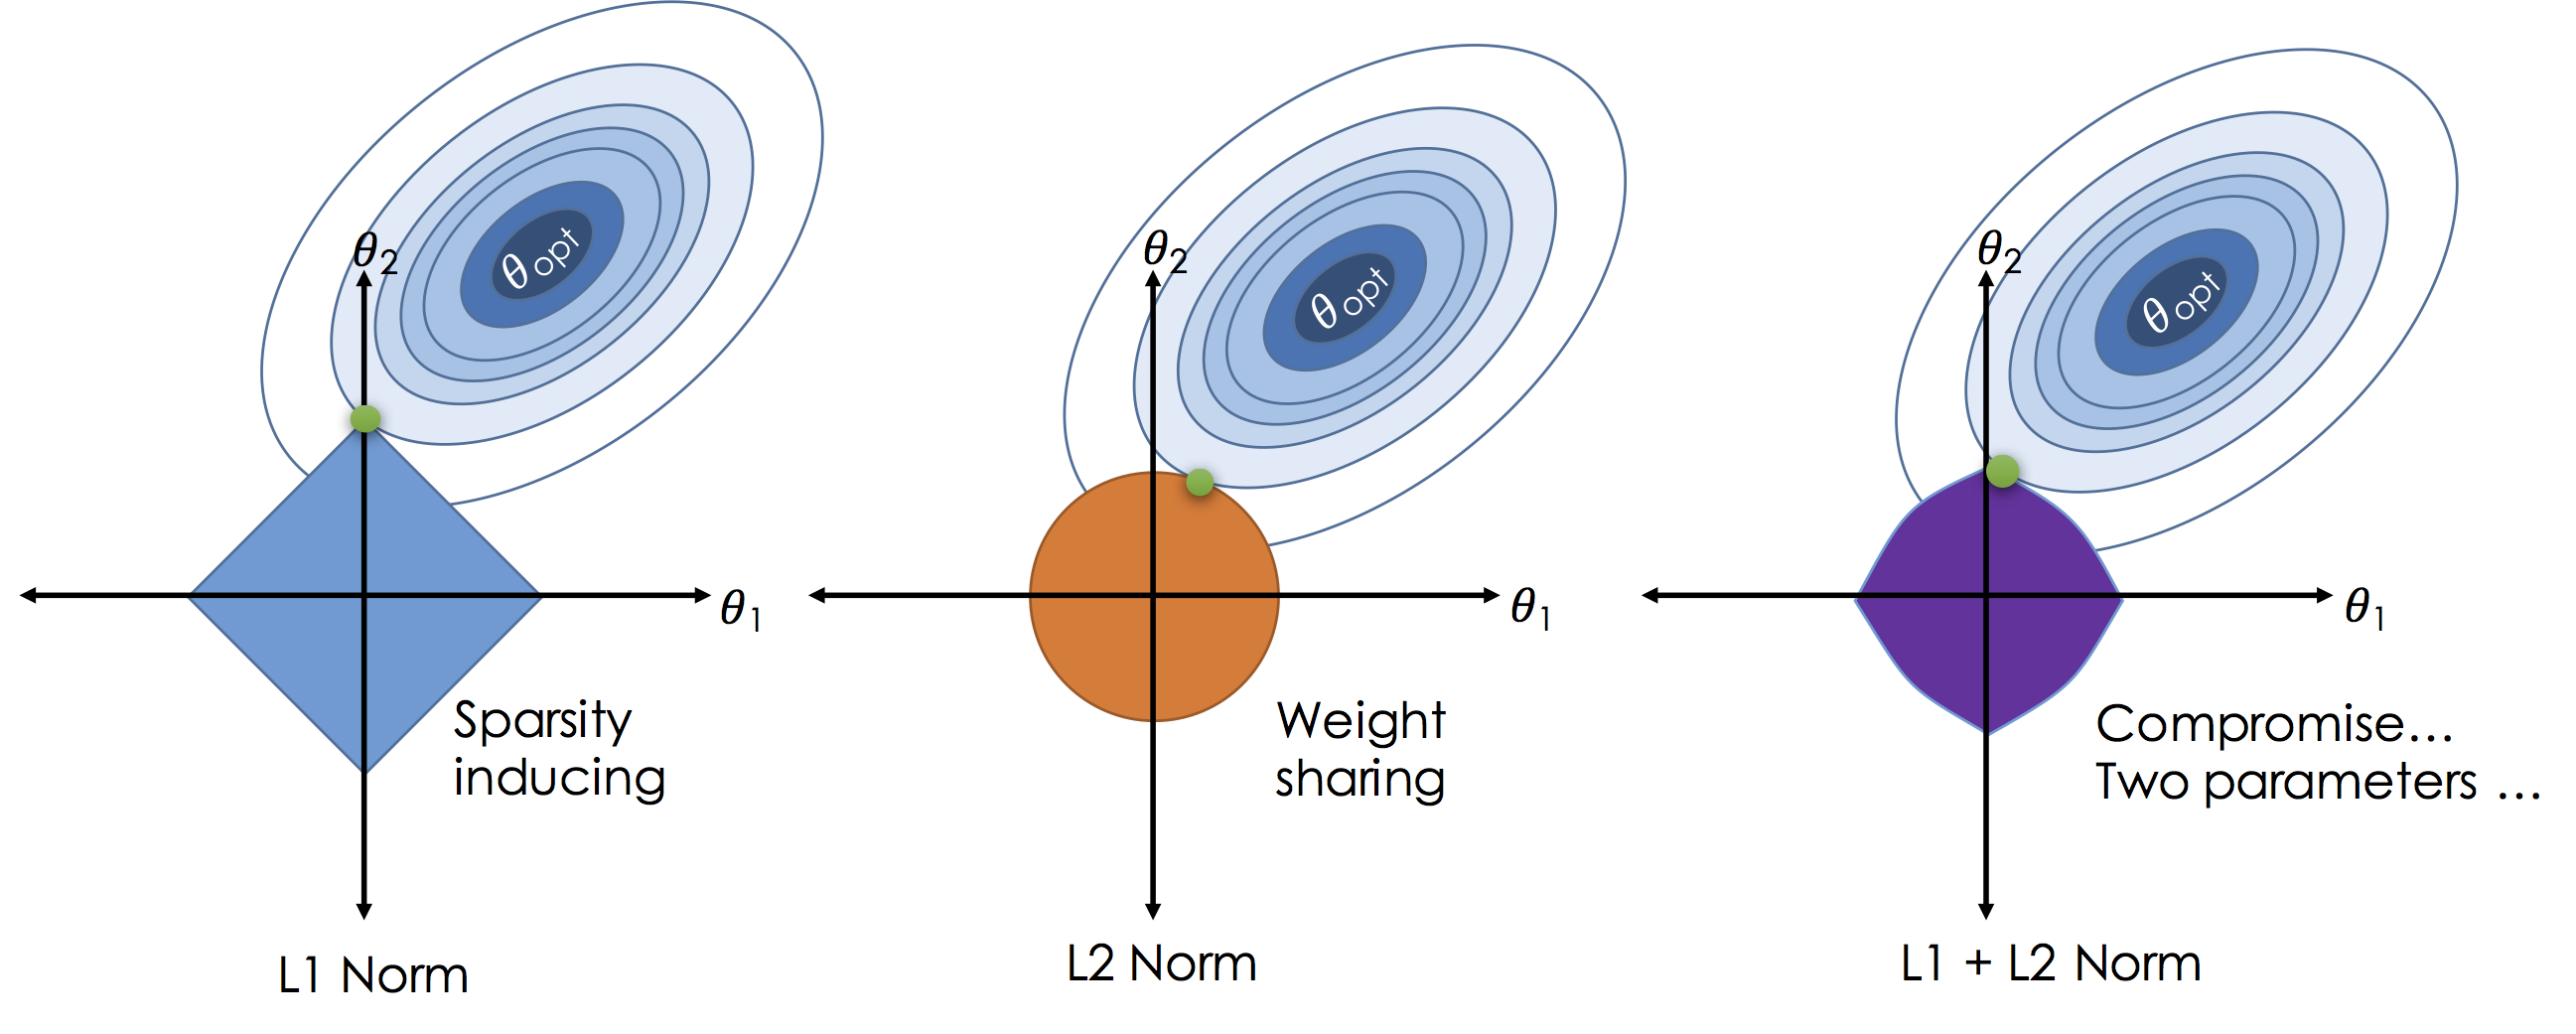
\includegraphics[width=\columnwidth]{norm_balls.png}
\end{center}

\vspace{-4mm}
\begin{flushright}
{\footnotesize \textcolor{gray}{Picture credit: 
http://www.ds100.org/sp17/assets/notebooks/linear\_regression/Regularization.html}}
\end{flushright}

\end{frame}



\begin{frame}
\frametitle{Another interpretation of regularizers}

\begin{figure}
\centering
\begin{minipage}{.5\textwidth}
  \centering
  
\includegraphics[width=0.6\columnwidth]{cat_source.png}
  \caption{\normalsize Large parameter space}
\end{minipage}%
\begin{minipage}{.5\textwidth}
  \centering
  
\includegraphics[width=0.85\columnwidth]{cat_regularized.png}
  \caption{\normalsize Regularized models}
\end{minipage}
\end{figure}

\end{frame}



\section{A~Bayesian~perspective on~regularization}



\begin{frame}
\frametitle{Principled definition of regularizers?}

\begin{itemize}

  \item \textbf{L2 regularized} linear regression
  \[
    \lVert \bm{y} - \bm{X} \mathbf{w}  \rVert^2 
    +
    \alpha \lVert \mathbf{w} \rVert^2 
    \to 
    \min_{\mathbf{w} \in \mathbb{R}^d}
  \]
  works better in some instances (many correlated features, etc.)

  \pause
  \item But why exactly we formulate penalty as $\alpha \lVert \mathbf{w} \rVert^2 $? 

  \pause
  \item Is there any \textbf{principled} way of defining regularizers?

  \pause
  \item Recall: we wanted $\mathbf{w}$ to take \textbf{small values} $\to \alpha$ controls how small they must be

  \pause
  \item In (Bayesian) statistics, \textbf{priors}
  are used to characterize variables
  with known (or assumed) distributions of values
  $\to$ use priors on weights $\mathbf{w}$!

\end{itemize}

\end{frame}



\begin{frame}
\frametitle{The prior and the posterior distributions}

\begin{itemize}
  \item $x$ is a mathematical entity
\end{itemize}

\pause
Questions:
\begin{itemize}

  \item What kinds of mathematical entities can have priors? 
  \item What is a prior for $x$?

\end{itemize}

\pause
Answers:
\begin{itemize}
  \item Prior probability distribution (\textbf{prior}): 
  ``the probability distribution that would express one's beliefs about this quantity before some evidence is taken into account.'' (wiki)

  \item Most mathematical objects can have priors

  \pause
  \item Sources: past experiments, expert assessment, \ldots

\end{itemize}


A typical scenario in Bayesian data analysis would be:\\
\begin{center}\noindent\fbox{%
    \parbox{25em}{%
design a prior $\to$ collect evidence (data) $\to$ compute a posterior
    }%
}
\end{center}

\end{frame}



\begin{frame}
\frametitle{Expressing prior knowledge using math}

\begin{itemize}

  \item How to technically impose the ``small values prior'' on $\mathbf{w}$? 

  \pause
  \item Let $P(\mathbf{w} < \varepsilon)$ be high,
  and $P(\mathbf{w} \geqslant \varepsilon)$ 
  be (exponentially) low $\to$ find a distribution
  that satisfies this condition

  \pause
  \item Example: Gaussian $\mathbf{w} \sim \mathcal{N}(0, \sigma^2 \bm{I})$


\end{itemize}



\end{frame}



\begin{frame}
\frametitle{Prior knowledge for linear regression}

\begin{itemize}

  \item Linear model for regression:
  \[
    \bm{y} = \bm{X} \mathbf{w} + \bm{\varepsilon}
    \implies
    y_i = f(x_i) + \varepsilon_i
  \]

  \pause
  \item Obtaining MLE for linear regression:

  \begin{itemize}
    \item $\bm{\varepsilon} \sim \mathcal{N}(0, \sigma^2_\varepsilon \bm{I})$;
    \item $\sigma^2_\varepsilon = \mathrm{const}$ (unknown);
    \item $\bm{\varepsilon}$ is \textbf{the only random variable}
  \end{itemize}

  \pause
  \item Likelihood for $\bm{\varepsilon}$:
  \[
  L = \prod_i P_\varepsilon(\varepsilon_i)
  \implies 
  \log L = -\sum_i \log P_\varepsilon(\varepsilon_i)
         = -\sum_i \log P_\varepsilon(y_i - f(x_i))
  \]

\end{itemize}
\end{frame}



\begin{frame}
\frametitle{Prior knowledge for linear regression}

\begin{itemize}

  \item MLE for $\mathbf{w}$...
  \begin{align*}
  L = &-\sum_i \log P_\varepsilon(y_i - f(x_i) ) = \\
      & \sum_i \left[ 
        Z(\sigma^2_\varepsilon) - 
        \frac{(y_i - f(x_i))^2}
             {2 \sigma^2_\varepsilon}
        \right] \sim \\
      & \sum_i (y_i - f(x_i))^2 \to 
        \min\limits_{\mathbf{w}}
        \implies \text{MSE problem!}
  \end{align*}

  \pause
  \item ...is \textbf{the same as the solution
  for the least squares problem} (with Gaussian errors)

\end{itemize}

\end{frame}




\begin{frame}
\frametitle{Prior knowledge for linear regression}

\begin{itemize}

  \item Data model:
  $\bm{\varepsilon} \sim \mathcal{N}(0, \sigma^2_\varepsilon\bm{I}).$

  \pause
  \item Weights prior: $\mathbf{w} \sim \mathcal{N}(0, \Sigma_w)$;

  \pause
  \item Computing posterior we get:
  \begin{align*}
    P(\mathbf{w} \mid \bm{y}, \bm{X}) 
        &\propto P(\bm{y} \mid \mathbf{w}, \bm{X}) P(\mathbf{w}) \\
        &\propto \exp\left[
            -\frac{1}{2 \sigma^2_\varepsilon} 
            (\bm{y} - \bm{X} \mathbf{w})^T (\bm{y} - \bm{X} \mathbf{w}) 
        \right] 
        \cdot 
        \exp\left[ 
            -\frac{1}{2} \mathbf{w}^T \Sigma^{-1}_w \mathbf{w} 
        \right] = \\
        &\propto \exp\left[ 
            -\frac{1}{2} (\mathbf{w} - \mathbf{w}^*)^T \bm{A}_w (\mathbf{w} - \mathbf{w}^*) 
        \right]
  \end{align*}
  where:
  \begin{itemize}
    \item $\bm{A}_w = 
        \frac{1}{\sigma^{2}_\varepsilon}\bm{X} \bm{X}^T + \Sigma^{-1}_w$;

    \item $\mathbf{w}^* = \frac{1}{\sigma^{2}_\varepsilon} \bm{A}^{-1}_w \bm{X} \bm{y}$.
  \end{itemize}
\end{itemize}

\end{frame}




% % \begin{frame}
% % \frametitle{}

% \section{Why~machine~learning~works:
% a~bit~of~learning~theory}


% % \end{frame}



% \begin{frame}
% \frametitle{Empirical Risk Minimization framework}

% \begin{itemize}
% \item Given a labeled sample $X^{\ell} = 
%     \big\{(\mathbf{x}_i, y_i)\big\}_{i=1}^{\ell}$
% and some candidate $h$

% \pause 
% \item Define the \textcolor{orange}{empirical error} of $h$ as
% $Q(h, X^{\ell}) = \frac {1} {\ell} 
% \sum\limits_{i=1} ^{\ell} 
%     [f(\mathbf{x}_i) \neq h(\mathbf{x}_i)]$\\
% (the proportion of sample points on which $h$ errs)

% \pause 
% \item $\mathrm{ERM}(X^{\ell})$ --- find $h$ the minimizes $Q(h, X^{\ell})$

% \pause 
% \item \textcolor{Fuchsia}{\textbf{No learning is possible without
% applying prior knowledge}}

% \pause 
% \item A hypothesis class $\mathbb{H}$ is a set of hypotheses

% \pause 
% \item Re-define the ERM rule by searching
% only inside such a prescribed $\mathbb{H}$

% \pause 
% \item $\mathrm{ERM}_{\mathbb{H}}(X^{\ell})$
% picks a classifier $h \in \mathbb{H}$
% that minimizes the empirical error over members of $\mathbb{H}$

% \end{itemize}

% \end{frame}



% \begin{frame}
% \frametitle{Guarantees for ERM}

% \begin{theorem}[Guaranteed success for $\mathrm{ERM}_{\mathbb{H}}$]
% \begin{itemize}
% \item Let $\mathbb{H}$ be a finite class.

% \item Let the unknown labeling rule,
% $f$, be a member of $\mathbb{H}$.

% \item Then 
% \begin{itemize}
% \item for every $\varepsilon, \delta > 0$, 
% if $m > (\log(|\mathbb{H}|) + \log(1/\delta))/ \varepsilon$,

% \item with probability $> 1 - \delta$ (over the choice of $X^{\ell}$),

% \item any $\mathrm{ERM}_{\mathbb{H}}$ hypothesis
% has error below $\varepsilon$.

% \end{itemize}

% \end{itemize}

% \end{theorem}

% \end{frame}


\end{document}
